\chapter{Provas de pertença à cadeia completa (FCMP++)}
\label{chapter:fcmp-plus-plus}
\label{page:fcmp-start}

Uma assinatura CLSAG diz, em conjunto, «uma destas dezasseis saídas é a minha,
conheço a sua chave e ainda não a gastei». FCMP++ desmonta essa frase e volta a
montá-la com um conjunto muitíssimo maior. Uma raiz curta passa a representar
todas as saídas admissíveis acumuladas pela cadeia; uma prova esconde o caminho
até à raiz; outra prova demonstra a autorização de gasto; e uma imagem de chave
determinística denuncia uma segunda tentativa de gastar a mesma saída.

O resultado é mais fácil de verificar do que de aprender, porque as fontes
começam frequentemente pela árvore. Faremos o contrário. Primeiro seguiremos
uma moeda desde a carteira de Alice até à decisão do nó. Só depois abriremos o
capot e veremos compromissos vectoriais, duas curvas, divisores e as equações
do verificador.

Curve Trees, de Matteo Campanelli, Mathias Hall-Andersen e Simon Holmgaard
Kamp, fornece o acumulador transparente e a prova do caminho oculto
\cite{curve-trees}. Liam Eagen fornece o método por divisores que torna
económicas certas multiplicações de curva dentro do circuito
\cite{eagen-divisors}. Luke «KayabaNerve» Parker adapta e compõe essas peças
para as tuplas de saída do Monero, acrescentando re-randomização, autorização
de gasto e ligação \cite{fcmp-plus-plus-paper}. Não há, portanto, um único
truque chamado FCMP++ nem um único autor de todas as peças.

\section{A pergunta certa: como demonstrar que uma saída é minha?}
\label{sec:fcmp-ownership-first}

Em linguagem corrente, Alice quer provar «esta saída é minha». Em linguagem
criptográfica, a palavra \emph{minha} decompõe-se em quatro afirmações:

\begin{enumerate}
 \item existe uma tupla de saída real no acumulador canónico;
 \item a tupla apresentada à prova é uma re-randomização dessa mesma saída;
 \item Alice conhece o segredo de utilização única que abre a chave da saída;
 \item a imagem de chave publicada é a que esse segredo determina para essa
 saída.
\end{enumerate}

A primeira e a segunda afirmações são a parte de \emph{pertença}. A terceira é
a \emph{autorização de gasto}. A quarta fornece \emph{ligação}: dois gastos da
mesma saída deixam o mesmo marcador, embora as provas tenham aleatoriedade
nova. O protocolo não certifica propriedade jurídica; certifica conhecimento
do segredo que o consenso aceita como autorização.

Quando Alice recebeu uma saída histórica, a sua carteira recuperou um escalar
secreto de utilização única. Chamá-lo-emos
\begin{align*}
 k_{\rm ligar}.
\end{align*}
Este nome será reservado ao segredo. Não o chamaremos \(x\), porque a letra
\(x\) também costuma designar a coordenada horizontal de um ponto e foi
exactamente assim que duas coisas sem parentesco acabaram na mesma frase.

A chave pública da saída admite a abertura geral
\begin{align}
 O=k_{\rm ligar}G+k_{\rm autor}T.
 \label{eq:fcmp-output-opening-semantic}
\end{align}
Para as saídas históricas, \(k_{\rm autor}=0\), logo
\(O=k_{\rm ligar}G\), e \(k_{\rm ligar}\) é a chave privada de utilização
única já conhecida dos capítulos anteriores. A abertura geral tem dois
coeficientes secretos. SAL abre \(\widetilde O\) com
\((k_{\rm ligar},\widetilde k_{\rm autor})\); FCMP prova a máscara que o liga
a \(O\). Só a composição demonstra a abertura autorizada original completa.
O coeficiente \(k_{\rm ligar}\) permanece ligado à imagem de chave. Esta
distinção também acomoda formatos e esquemas de multi-assinatura futuros sem
baptizar qualquer coordenada geométrica de «chave».

No caso histórico, \(k_{\rm ligar}\) é a mesma chave privada de saída, única,
que a carteira usaria na CLSAG; não é uma coordenada, nem a chave permanente
da conta, nem um segredo novo criado pela FCMP++.

A cadeia acumula uma folha ordenada
\begin{align}
 \mathsf{Folha}_j=(O_j,I_j,C_j),
 \label{eq:fcmp-leaf-semantic}
\end{align}
onde \(I_j\) é a base da imagem de chave derivada da chave pública original e
\(C_j\) é o compromisso de montante. A imagem de chave só aparece ao gastar:
\begin{align}
 K_{\rm imagem}=k_{\rm ligar}I_j.
 \label{eq:fcmp-key-image-semantic}
\end{align}
O código corrente chama a este ponto \texttt{L}; aqui damos-lhe um nome que
diz o que faz e reservamos \(\mathsf{Folha}\) às folhas da árvore.

\begin{center}
\renewcommand{\arraystretch}{1.25}
\begin{tabular}{|l|c|p{5.9cm}|}
 \hline
 \textbf{objecto} & \textbf{tipo} & \textbf{papel}\\
 \hline
 \(k_{\rm ligar},k_{\rm autor}\) & escalares secretos & abertura autorizada
 de \(O\); o primeiro determina a imagem de chave\\
 \hline
 \(O,I,C\) & três pontos & dados da saída que formam uma folha\\
 \hline
 \(\mathcal R_{\rm tree}\) & ponto público & resumo de um estado do conjunto de
 folhas\\
 \hline
 \(K_{\rm imagem}\) & ponto público & marcador determinístico de gasto duplo\\
 \hline
\end{tabular}
\end{center}

Já podemos responder à pergunta central numa linha:
\begin{align*}
 \boxed{\text{pertença da folha}}
 \quad+\quad
 \boxed{\text{conhecimento da abertura de }O}
 \\
 {}+\quad
 \boxed{K_{\rm imagem}=k_{\rm ligar}I}
 \quad=\quad
 \boxed{\text{autorização FCMP++ completa}}.
\end{align*}
Nenhuma das três caixas basta isoladamente. Qualquer observador conhece folhas
da cadeia; isso não lhe dá a abertura secreta. Qualquer pessoa pode inventar uma
chave e demonstrar que conhece o respectivo segredo; isso não põe a chave na
árvore. E um marcador sem ligação às duas provas seria apenas mais um ponto.

\section{Pontos, coordenadas, rótulos e chaves privadas}
\label{sec:fcmp-coordinates-not-keys}

Antes da árvore, precisamos de uma quarentena tipográfica. Um ponto afim será
sempre escrito
\begin{align}
 P=(P_{\rm hor},P_{\rm ver}),
 \qquad
 \operatorname{hor}(P)=P_{\rm hor},
 \qquad
 \operatorname{ver}(P)=P_{\rm ver}.
 \label{eq:fcmp-coordinate-convention}
\end{align}
\(P\) é um ponto; \(P_{\rm hor}\) e \(P_{\rm ver}\) são elementos do campo.
Nenhum dos dois é, por esse facto, a chave privada que multiplicou um gerador
para produzir \(P\).

No modelo de Weierstrass usado pelo dispositivo de divisores, as coordenadas
satisfazem
\begin{align}
 P_{\rm ver}^{\,2}
   =P_{\rm hor}^{\,3}
    +a_{\rm curva}P_{\rm hor}+b_{\rm curva},
 \label{eq:fcmp-point-coordinate-equation}
\end{align}
onde \(a_{\rm curva}\) e \(b_{\rm curva}\) são coeficientes públicos fixos da
curva.
Fixar um valor horizontal não inventa automaticamente um ponto. O lado direito
pode não ter raiz quadrada no campo. Quando tem e a raiz não é zero, há em
geral duas escolhas verticais, \(P_{\rm ver}\) e \(-P_{\rm ver}\). Assim,
\begin{align*}
 \operatorname{hor}(P)\quad
 &\text{não determina sozinho o ponto completo},\\
 P=(P_{\rm hor},P_{\rm ver})\quad
 &\text{já traz uma coordenada vertical válida}.
\end{align*}

Esta é a resposta directa à expressão da imagem, escrita ali com uma função
chamada «x» diante do ponto indexado por nível. Ela não significa «o segredo
de gasto aplicado a uma chave» nem «uma coordenada vertical ainda por
descobrir». Reescrevê-la-emos sem a colisão:
\begin{align}
 \underbrace{P_{n,j}=(P^{\rm hor}_{n,j},P^{\rm ver}_{n,j})}_
             {\text{ponto completo no nível }n}
 \quad\xrightarrow{\ \operatorname{hor}\ }\quad
 \underbrace{\operatorname{hor}(P_{n,j})=P^{\rm hor}_{n,j}}_
             {\text{rótulo escalar guardado no pai}}.
 \label{eq:fcmp-point-to-parent-label}
\end{align}
O ponto completo existe primeiro. O circuito conserva as duas coordenadas,
verifica a equação da curva e liga o ponto ao compromisso do ramo anterior.
Só o pai guarda a coordenada horizontal como rótulo curto. Portanto, sim: a
coordenada vertical daquele ponto existe e faz parte da testemunha; não, o
rótulo horizontal sozinho não escolhe de modo único entre os dois sinais.

A diferença para uma chave privada vê-se melhor sem árvores. Se
\begin{align*}
 O=k_{\rm ligar}G,
\end{align*}
o ponto público \(O=(O_{\rm hor},O_{\rm ver})\) e ambas as coordenadas podem
ser conhecidos por toda a gente. O segredo é o \emph{coeficiente}
\(k_{\rm ligar}\). Recuperá-lo de \(G\) e \(O\) é o problema do logaritmo
discreto. Coordenadas dizem onde está o ponto; a chave privada diz quantos
passos escalares, no sentido da operação de grupo, o relacionam com a base.

\begin{center}
\begin{tikzpicture}[node distance=1.35cm and 1.4cm,
 box/.style={rectangle,rounded corners,draw=black,align=center,
   minimum height=1.0cm,text width=4.0cm}]
 \node[box,fill=yellow!22] (secret)
   {\(k_{\rm ligar}\)\\escalar secreto da carteira};
 \node[box,fill=green!18,right=of secret] (output)
   {\(O=k_{\rm ligar}G\)\\ponto público de uma saída histórica};
 \node[box,fill=blue!12,below=of output] (coords)
   {\((O_{\rm hor},O_{\rm ver})\)\\coordenadas públicas do ponto};
 \draw[->,thick] (secret) -- node[above]{multiplicação escalar} (output);
 \draw[->,thick] (output) -- node[right]{representação afim} (coords);
 \draw[->,thick,dashed] (coords) -- node[below left,align=right]
   {logaritmo discreto\\considerado inviável} (secret);
\end{tikzpicture}
\end{center}

Daqui em diante, \(\operatorname{hor}(P)\) será sempre uma coordenada,
\(k_{\rm ligar}\) será sempre o segredo que determina a imagem de chave,
\(k_{\rm autor}\) o segundo coeficiente da abertura e \(m_{\rm algo}\) será
sempre uma máscara aleatória cujo índice diz o que ela oculta. O alfabeto já
tem trabalho suficiente; não lhe pediremos que adivinhe tipos.

\section{A prova inteira, uma vez, de ponta a ponta}
\label{sec:fcmp-first-end-to-end}

Alice conhece \(k_{\rm ligar}\), \(k_{\rm autor}\) e os dados necessários à
sua saída \(\mathsf{Folha}_j=(O,I,C)\). Quando a quer gastar, acontece o
seguinte.

\begin{enumerate}
 \item A carteira escolhe máscaras novas e transforma a folha. A entrada
 pública re-randomizada é
 \begin{align*}
  (\widetilde O,\widetilde I,R_{\rm ligar},\widetilde C).
 \end{align*}
 Esses quatro pontos não podem ser procurados directamente na árvore.

 \item A prova FCMP abre esses pontos \emph{dentro do circuito}, recupera
 \((O,I,C)\) sem os revelar, demonstra que os três pontos ocupam juntos uma
 folha e sobe por um caminho escondido até \(\mathcal R_{\rm tree}\).

 \item A prova SAL recebe a mesma entrada re-randomizada. Demonstra que Alice
 conhece \(k_{\rm ligar}\) e
 \(\widetilde k_{\rm autor}=k_{\rm autor}+m_O\), que abrem
 \(\widetilde O\), e usa \(m_I\) nas suas relações. É a FCMP que prova, para
 a mesma entrada, \(\widetilde O=O+m_OT\) e
 \(\widetilde I=I+m_IU\). Juntas, recuperam a abertura original sem a
 publicar.

 \item SAL publica
 \begin{align*}
  K_{\rm imagem}=k_{\rm ligar}I,
 \end{align*}
 mas calcula-o a partir de \(\widetilde I\), sem revelar \(I\). O compromisso
 \(R_{\rm ligar}\) obriga FCMP e SAL a usarem a mesma máscara.

 \item As regras RingCT verificam o equilíbrio dos compromissos de montante e
 a restante validade da transacção. O nó rejeita ainda
 \(K_{\rm imagem}\) se esse ponto já tiver aparecido.
\end{enumerate}

\begin{center}
\begin{tikzpicture}[node distance=1.05cm and .55cm,
 flow/.style={rectangle,rounded corners,draw=black,align=center,
   minimum height=.9cm,text width=4.4cm,font=\small}]
 \node[flow,fill=green!18] (wallet)
   {carteira: abertura secreta de \(O\) e uma folha real \((O,I,C)\)};
 \node[flow,fill=yellow!22,below=of wallet] (mask)
   {máscaras novas: \((\widetilde O,\widetilde I,
      R_{\rm ligar},\widetilde C)\)};
 \node[flow,fill=blue!12,below left=of mask,xshift=-.3cm] (member)
   {FCMP\\a entrada abre para uma folha sob a raiz};
 \node[flow,fill=blue!12,below right=of mask,xshift=.3cm] (auth)
   {SAL\\conheço a abertura e derivo \(K_{\rm imagem}\)};
 \node[flow,fill=green!18,below=2.7cm of mask] (accept)
   {nó: mesma entrada nas duas provas + equilíbrio + imagem de chave nova};
 \draw[->,thick] (wallet) -- (mask);
 \draw[->,thick] (mask) -- (member);
 \draw[->,thick] (mask) -- (auth);
 \draw[->,thick] (member) -- (accept);
 \draw[->,thick] (auth) -- (accept);
\end{tikzpicture}
\end{center}

O ponto decisivo é a interface comum. FCMP, sozinho, pode provar pertença de
uma saída alheia: as folhas são públicas. SAL, sozinha, pode autorizar uma
chave inventada que nunca recebeu moeda. A composição exige que ambas falem
dos mesmos quatro pontos re-randomizados. É nessa costura, e não numa vaga
semelhança visual, que «está na cadeia» se torna «está na cadeia e conheço o
segredo que a gasta».

\subsection{Três pontos que as fontes chamam \texorpdfstring{\(R\)}{R}}
\label{sec:fcmp-three-rs}

Há ainda uma colisão que eliminaremos antes de avançar:
\begin{align*}
 \mathcal R_{\rm tree}
   &:\quad \text{raiz pública e persistente da Curve Tree},\\
 R_{\rm nonce}
   &:\quad \text{compromisso efémero de uma prova Schnorr},\\
 R_{\rm ligar}
   &:\quad \text{compromisso que costura FCMP a SAL}.
\end{align*}
O primeiro resume um estado da cadeia. O segundo nasce e morre numa prova. O
terceiro acompanha uma entrada e compromete a máscara de \(I\). Mais tarde
derivaremos cada equação; por agora basta não deixar três objectos vestir o
mesmo sobretudo.

\section{Do anel explícito ao acumulador Curve Trees}
\label{sec:fcmp-ring-to-tree}

Uma assinatura em anel parte de uma lista explícita
\begin{align*}
 \mathcal S=(M_0,M_1,\ldots,M_{N-1})
\end{align*}
e prova uma disjunção:
\begin{align*}
 \text{conheço a abertura de }M_0
 \quad\mathbf{OU}\quad\cdots\quad\mathbf{OU}\quad
 \text{conheço a abertura de }M_{N-1}.
\end{align*}
O custo mais ingénuo cresce com \(N\). Técnicas melhores comprimem a prova,
mas o verificador ainda precisa de saber qual é a lista que a declaração
designa. Com FCMP, o tamanho dessa lista cresce com o número de saídas e muda
sempre que entram saídas novas.

Um \emph{acumulador} substitui a lista por um resumo curto. Queremos três
operações:

\begin{enumerate}
 \item \textbf{acumular}: transformar muitos membros num valor público curto;
 \item \textbf{testemunhar}: obter informação privada que liga um membro ao
 resumo;
 \item \textbf{provar}: convencer um verificador da ligação sem revelar o
 membro nem a posição.
\end{enumerate}

Uma árvore de Merkle resolve as duas primeiras operações. A raiz
resume as folhas e um caminho de hashes autentica uma folha. Mas um caminho de
Merkle normal revela a folha, o índice e os irmãos. Colocá-lo dentro de um
circuito de conhecimento zero é possível, mas as funções hash adequadas a bytes
não são necessariamente económicas na aritmética de curvas que já estamos a
usar.

Em Curve Trees, cada nó é um compromisso de Pedersen
\emph{vectorial} aos filhos. As relações do caminho podem assim ser expressas
directamente no circuito dos Bulletproofs. Cada nível verifica a afirmação:

\begin{center}
\(\text{«este ponto, depois de ofuscado, é um dos pontos comprometidos
naquele pai.»}\)
\end{center}

\section{Compromissos vectoriais dos nós}
\label{sec:fcmp-vector-commitment}

Já conhecemos o compromisso de Pedersen com duas bases,
\begin{align*}
 C=a_{\rm mont}G+v_{\rm mont}H.
\end{align*}
Um compromisso vectorial oferece uma base por coordenada. Para o vector
\(\mathbf v=(v_0,\ldots,v_{n-1})\), escrevemos
\begin{align}
 \operatorname{Com}(\mathbf v;m_{\text{nó}})
   =m_{\text{nó}}H+\sum_{j=0}^{n-1}v_jG_j
   =m_{\text{nó}}H+\langle\mathbf v,\mathbf G\rangle.
 \label{eq:fcmp-vector-commitment}
\end{align}
O escalar \(m_{\text{nó}}\) esconde a abertura. A família
\((H,G_0,\ldots,G_{n-1})\) é pública e não deve ter relações de logaritmo
discreto conhecidas. Se alguém soubesse coeficientes não todos nulos cuja
combinação desse a identidade, poderia calcular aberturas alternativas para o
mesmo compromisso. É a generalização multibase da independência entre bases
que já exigimos para compromissos de montante na secção \ref{gamma}; não
precisamos de dar uma letra ao logaritmo que ninguém deve conhecer.

Esta é a máquina de compromisso genérica usada pela prova, não ainda a
codificação canónica de um nó público. A árvore substitui a máscara secreta
por um inicializador fixo \(J_{\rm init}\); durante a prova, máscaras novas
ofuscam os pontos transportados. Assim \(m_{\text{nó}}\) pertence à abertura
oculta, enquanto \(J_{\rm init}\) pertence ao hash determinístico abaixo.

Nas camadas superiores há dois objectos que não devem receber o mesmo nome. O
caminho transporta um ponto completo; o ramo do pai guarda apenas a sua
coordenada horizontal como rótulo escalar:
\begin{align*}
 \underbrace{P_{n,j}=(P^{\rm hor}_{n,j},P^{\rm ver}_{n,j})}_
             {\text{ponto que sobe e pode ser ofuscado}}
 \quad\xrightarrow{\ \operatorname{hor}\ }\quad
 \underbrace{\operatorname{hor}(P_{n,j})=P^{\rm hor}_{n,j}}_
             {\text{escalar guardado no pai}},
 \qquad n\geq1.
\end{align*}
O primeiro índice marca o nível; o segundo marca a posição local dentro de um
pai. Na construção actual, um ramo superior é portanto
\begin{align*}
 \underbrace{\mathcal B_n=
   \bigl(\operatorname{hor}(P_{n,0}),\ldots,
         \operatorname{hor}(P_{n,m-1})\bigr)}_
   {\substack{\text{um ramo: }m\text{ rótulos}\\
              \text{dos irmãos no nível }n}}
 \quad\xrightarrow{\ \operatorname{Com}_{n\to n+1}\ }\quad
 \underbrace{P^{\rm pai}_{n+1}}_{\text{um ponto no nível }n+1}.
\end{align*}
Na primeira camada há a única excepção tipográfica: as entradas de
\(\mathcal B_0\) são folhas completas
\(\mathsf{Folha}_j=(O_j,I_j,C_j)\), não coordenadas isoladas.

Um ramo \(\mathcal B_n\) é a lista ordenada das entradas associadas aos
filhos de \emph{um} pai; não é o nível inteiro nem o trajecto da folha à raiz.
Para \(n\geq1\), essas entradas são rótulos escalares, e os colchetes
escolhem o rótulo de uma posição:
\begin{align}
 \boxed{\mathcal B_n[j]=\operatorname{hor}(P_{n,j})}.
 \label{eq:fcmp-branch-slot}
\end{align}
O circuito conserva também o ponto completo \(P_{n,j}\): precisa dele
para verificar que está na curva e para produzir a sua representação
ofuscada. O pai canónico, omitindo apenas notação de curvas, é
\begin{align}
 P^{\rm pai}_{n+1}
   =\operatorname{Com}_{n\to n+1}(\mathcal B_n)
   =J^{n+1}_{\rm init}
    +\sum_{j=0}^{m-1}\operatorname{hor}(P_{n,j})G^{n+1}_j.
 \label{eq:curve-tree-parent}
\end{align}

Aqui a comutatividade não apaga as posições:
\begin{align*}
 \text{reordenar as parcelas:}\quad
 \operatorname{hor}(P_{n,0})G_0+\operatorname{hor}(P_{n,1})G_1
 &=\operatorname{hor}(P_{n,1})G_1+\operatorname{hor}(P_{n,0})G_0,\\
 \text{permutar os filhos:}\quad
 \operatorname{hor}(P_{n,0})G_0+\operatorname{hor}(P_{n,1})G_1
 &\underset{\text{em geral}}{\ne}
 \operatorname{hor}(P_{n,1})G_0+\operatorname{hor}(P_{n,0})G_1.
\end{align*}
Na primeira linha, cada escalar continua emparelhado com o seu gerador; na
segunda, os rótulos trocaram de posição. Depois de fixada a raiz, não se
baralha \(\mathcal B_n\): a prova esconde a posição, não reordena o ramo.

Um caminho atravessa níveis. O compromisso de um ramo produz o ponto que sobe;
o ramo seguinte guarda a sua coordenada horizontal numa posição possivelmente
diferente:
\begin{align}
 \boxed{
 P^{\rm pai}_{n+1}=P_{n+1,j_{n+1}}
 \quad\Longrightarrow\quad
 \mathcal B_{n+1}[j_{n+1}]=\operatorname{hor}(P^{\rm pai}_{n+1})}.
 \label{eq:curve-tree-parent-becomes-child}
\end{align}

\subsection{Um único exemplo: árvore ternária de profundidade três}
\label{sec:fcmp-running-example}

Usaremos o mesmo exemplo até ao fim da explicação do caminho. A ramificação
\(m=3\) é deliberadamente pequena para tornar os índices visíveis; a
implementação usa larguras 38 e 18, mas repete exactamente o mesmo padrão:
ponto \(\to\) coordenada horizontal \(\to\) ramo.
Com profundidade \(d=3\), a árvore comporta
\begin{align*}
 27=3^3
\end{align*}
folhas sem precisar de desenhar vinte e sete caixas.

Abreviaremos \(\mathsf{Folha}_r\) por \(\mathsf F_r\). Os pontos que sobem
chamar-se-ão \(P_j\) e \(Q_k\); o sobrescrito \({\rm hor}\) mostrará
explicitamente quando usamos só a coordenada guardada no ramo seguinte:
\begin{align*}
 \mathsf F_r&=(O_r,I_r,C_r),\qquad 0\leq r<27,\\
 P_j&=\operatorname{Com}_{0\to1}
   (\mathsf F_{3j},\mathsf F_{3j+1},\mathsf F_{3j+2}),
 &P_j^{\rm hor}&:=\operatorname{hor}(P_j),&0&\leq j<9,\\
 Q_k&=\operatorname{Com}_{1\to2}
   (P_{3k}^{\rm hor},P_{3k+1}^{\rm hor},P_{3k+2}^{\rm hor}),
 &Q_k^{\rm hor}&:=\operatorname{hor}(Q_k),&0&\leq k<3,\\
 \mathcal R_{\rm tree}
 &=\operatorname{Com}_{2\to3}
   (Q_0^{\rm hor},Q_1^{\rm hor},Q_2^{\rm hor}).
\end{align*}
Cada folha fornece três pontos \((O,I,C)\), duas coordenadas por ponto. As
setas seguintes são projecções de coordenada, não mudanças de nome:
\begin{align*}
 \boxed{P_j\text{ é um ponto}}
 &\xrightarrow{\ \operatorname{hor}\ }
 \boxed{P_j^{\rm hor}\text{ é um escalar}},\\
 \boxed{Q_k\text{ é um ponto}}
 &\xrightarrow{\ \operatorname{hor}\ }
 \boxed{Q_k^{\rm hor}\text{ é um escalar}}.
\end{align*}

No desenho, mostramos o caminho e, em cada altura, os irmãos locais; só o nó
escolhido é expandido. As caixas cinzentas com \(\vdots\) condensam subárvores
fora do caminho:

\begin{center}
\begin{forest}
for tree={draw,rounded corners,align=center,l sep=1.05cm,s sep=.18cm,
  font=\small}
[\(\mathcal R_{\rm tree}\),fill=blue!12
  [{\(Q_0\)\\\(\vdots\)\\{\scriptsize\(\mathsf F_0,\ldots,\mathsf F_8\)}},fill=black!10,
    draw=black!55,dashed,edge={draw=black!40,dashed}]
  [{\(Q_1\)\\\(\vdots\)\\{\scriptsize\(\mathsf F_9,\ldots,\mathsf F_{17}\)}},fill=black!10,
    draw=black!55,dashed,edge={draw=black!40,dashed}]
  [\(Q_2\),fill=green!18,edge={very thick,blue!65!black}
    [{\(P_6\)\\\(\vdots\)\\{\scriptsize\(\mathsf F_{18},\ldots,\mathsf F_{20}\)}},fill=black!10,
      draw=black!55,dashed,edge={draw=black!40,dashed}]
    [\(P_7\),fill=green!18,edge={very thick,blue!65!black}
      [\(\mathsf F_{21}\),fill=yellow!25,edge={very thick,blue!65!black}]
      [\(\mathsf F_{22}\)]
      [\(\mathsf F_{23}\)]]
    [{\(P_8\)\\\(\vdots\)\\{\scriptsize\(\mathsf F_{24},\ldots,\mathsf F_{26}\)}},fill=black!10,
      draw=black!55,dashed,edge={draw=black!40,dashed}]]]
\end{forest}
\end{center}

Cada grupo de irmãos determina um ramo local; acima do nível \(0\), esse ramo
guarda as coordenadas horizontais, não os pontos completos. A cadeia de arestas
azuis, atravessando níveis, é o caminho da folha à raiz.

O número da folha já contém o caminho. Como
\begin{align*}
 21=(210)_3,
 \qquad
 \underbrace{2\longrightarrow1\longrightarrow0}_{\text{da raiz à folha}},
 \qquad
 \underbrace{0\longrightarrow1\longrightarrow2}_{\text{da folha à raiz}},
\end{align*}
\(\mathsf F_{21}\) ocupa a posição \(0\) no seu ramo, o ponto \(P_7\) fornece o
rótulo da posição \(1\) no ramo seguinte e \(Q_2\) fornece o rótulo da posição
\(2\) junto à raiz. As quatro linhas são
\begin{align*}
 \mathcal B_0&=(\mathsf F_{21},\mathsf F_{22},\mathsf F_{23}),
 &\mathcal B_0[0]&=\mathsf F_{21}=(O_{21},I_{21},C_{21}),\\
 \operatorname{Com}_{0\to1}(\mathcal B_0)&=P_7,
 &\mathcal B_1&=(P_6^{\rm hor},\boxed{P_7^{\rm hor}},P_8^{\rm hor}),\\
 \operatorname{Com}_{1\to2}(\mathcal B_1)&=Q_2,
 &\mathcal B_2&=(Q_0^{\rm hor},Q_1^{\rm hor},\boxed{Q_2^{\rm hor}}),\\
 \operatorname{Com}_{2\to3}(\mathcal B_2)&=\mathcal R_{\rm tree}.&&
\end{align*}
Esta é a distinção que importa: \(P_7\ne\mathcal B_1[1]\), porque o lado
esquerdo é um ponto e o ramo guarda o escalar
\(P_7^{\rm hor}=\operatorname{hor}(P_7)=\mathcal B_1[1]\). Do mesmo modo,
\(Q_2^{\rm hor}=\operatorname{hor}(Q_2)=\mathcal B_2[2]\). A prova esconde as três posições
\((0,1,2)\) e a folha, sem representar os outros vinte e seis caminhos.

Em geral, uma árvore \(m\)-ária completa de profundidade \(d\) tem capacidade
\begin{align*}
 N=m^d,
 \qquad d=\log_mN.
\end{align*}
Cada nível ainda exige restrições sobre um ramo com \(m\) posições, mas o
caminho cresce com \(d\), não com a cadeia completa.

\subsubsection*{A raiz não é recalculada do zero}

Voltemos agora a um instantâneo anterior da mesma árvore. As folhas até
\(\mathsf F_{21}\) já existem e chega a saída real \(\mathsf F_{22}\). Apenas uma posição do
ramo activo muda:
\begin{align*}
\begin{array}{r@{\qquad}c@{\qquad}c@{\qquad}c@{\qquad}l}
 \text{posição global da folha}&21&\boxed{22}&23&\text{resumo}\\
 \mathcal B_0\text{ antes}&\mathsf F_{21}&\square&\square&\Longrightarrow P_7\\
 \mathcal B_0\text{ depois}&\mathsf F_{21}&\mathsf F_{22}&\square&\Longrightarrow P_7'
\end{array}
\end{align*}
Na linha ``antes'', \(\mathsf F_{22}\) e \(\mathsf F_{23}\) ainda não existem; na linha
``depois'', apenas \(\mathsf F_{22}\) passou a existir. Os \(\square\) não são saídas
fictícias usadas numa transacção: são enchimento zero, contribuem
\(0\mathbin{\cdot}G_j=\mathbf 0\) e não podem ser seleccionados nem gastos.
A saída real substitui \(\square\) pela folha completa
\(\mathsf F_{22}=(O_{22},I_{22},C_{22})\).

O novo índice confirma quais colunas mudam:
\begin{align*}
 22=(211)_3,
 \qquad
 \underbrace{1\longrightarrow1\longrightarrow2}_
             {\text{posições actualizadas, da folha à raiz}}.
\end{align*}
Este não é o caminho secreto anterior \((0,1,2)\) de \(\mathsf F_{21}\). A nova
folha escolhe a posição \(1\) dentro de \(\mathcal B_0\), mas partilha com
\(\mathsf F_{21}\) as posições superiores \(1\) e \(2\); por isso actualiza os mesmos
antepassados \(P_7\) e \(Q_2\).

O ponto mudou, logo muda o seu rótulo
\(P_7^{\rm hor}=\operatorname{hor}(P_7)\mapsto
{P_7'}^{\rm hor}=\operatorname{hor}(P_7')\). Esse único escalar ocupa a mesma posição
\(1\) no ramo seguinte:
\begin{align*}
\begin{array}{r@{\qquad}c@{\qquad}c@{\qquad}c@{\qquad}l}
 \text{posição dentro de }Q_2&0&\boxed{1}&2&\text{resumo}\\
 \mathcal B_1\text{ antes}&P_6^{\rm hor}&P_7^{\rm hor}&\square&\Longrightarrow Q_2\\
 \mathcal B_1\text{ depois}&P_6^{\rm hor}&{P_7'}^{\rm hor}&\square&\Longrightarrow Q_2'
\end{array}
\end{align*}
Finalmente, \(Q_2^{\rm hor}=\operatorname{hor}(Q_2)\mapsto
{Q_2'}^{\rm hor}=\operatorname{hor}(Q_2')\) altera a posição \(2\) do
ramo da raiz:
\begin{align*}
\begin{array}{r@{\qquad}c@{\qquad}c@{\qquad}c@{\qquad}l}
 \text{posição dentro da raiz}&0&1&\boxed{2}&\text{raiz}\\
 \mathcal B_2\text{ antes}&Q_0^{\rm hor}&Q_1^{\rm hor}&Q_2^{\rm hor}
   &\Longrightarrow\mathcal R_{\rm tree}\\
 \mathcal B_2\text{ depois}&Q_0^{\rm hor}&Q_1^{\rm hor}&{Q_2'}^{\rm hor}
   &\Longrightarrow\mathcal R'_{\rm tree}
\end{array}
\end{align*}
Nada se desloca e nada se baralha. O caminho actualizado lê-se nas três
colunas em caixa:
\begin{align*}
 \square&\mapsto\mathsf F_{22}
 \Longrightarrow P_7\mapsto P_7'
 \xrightarrow{\ \operatorname{hor}\ }P_7^{\rm hor}\mapsto {P_7'}^{\rm hor}\\
 &\Longrightarrow Q_2\mapsto Q_2'
 \xrightarrow{\ \operatorname{hor}\ }Q_2^{\rm hor}\mapsto {Q_2'}^{\rm hor}
 \Longrightarrow\mathcal R_{\rm tree}\mapsto\mathcal R'_{\rm tree}.
\end{align*}
Todos os ramos fora desta linha ficam guardados e são reutilizados.

Pela linearidade, o compromisso guardado recebe apenas a diferença da posição
alterada. Neste exemplo de profundidade três, a chegada de \(\mathsf F_{22}\) custa
\begin{align*}
 \underbrace{2+2+2}_{O_{22},\ I_{22},\ C_{22}}
 +\underbrace{1}_{{P_7'}^{\rm hor}\text{ em }\mathcal B_1}
 +\underbrace{1}_{{Q_2'}^{\rm hor}\text{ em }\mathcal B_2}
 &=8\quad\text{termos escalar--ponto}.
\end{align*}
Em profundidade \(d\), o mesmo padrão é
\begin{align*}
 \underbrace{2+2+2}_{O,\ I,\ C}
 +\underbrace{(d-1)}_{\text{um rótulo por camada superior}}
 &=d+5,\\
 \boxed{\text{trabalho incremental}}
 &\text{ é proporcional a }d=\log_mN,\\
 &\text{não a }N.
\end{align*}
Aqui são três actualizações de hash/adições de grupo e duas extracções de
coordenada horizontal. Ainda não há transporte: \(\mathsf F_{23}\) completa \(P_7\),
\(\mathsf F_{24}\) abre o irmão \(P_8\), e só \(\mathsf F_{27}\) excede esta árvore de
profundidade três e força uma nova camada.

As folhas não sobem. Dentro de cada instantâneo ficam todas na camada de base;
o que se propaga para cima são apenas os pontos-resumo e, depois, os seus
rótulos horizontais. Ao esgotar a capacidade do topo, acrescenta-se uma nova raiz
acima da árvore anterior. A profundidade é portanto fixa para um instantâneo,
mas não para toda a vida da cadeia.

Os pontos geradores fixos são preparados uma vez, e tabelas de base fixa são
uma optimização possível. O que se pré-calcula é o estado conhecido: resumos
dos ramos e fronteira activa. Folhas ainda desconhecidas não podem ser
pré-calculadas. Conservar os ramos necessários às testemunhas acrescenta
armazenamento e E/S, separados da aritmética acima. Ao verificar um gasto, o
nó verifica a prova contra a raiz guardada; não reconstrói a árvore. A
Secção~\ref{sec:fcmp-tree-growth} formaliza esta actualização.

\section{Selecção privada e re-randomização}
\label{sec:fcmp-select-rerandomize}

No exemplo ternário, os três ramos do caminho são
\begin{align*}
 \mathcal B_0&=(\mathsf F_{21},\mathsf F_{22},\mathsf F_{23}),&j_0&=0,\\
 \mathcal B_1&=(P_6^{\rm hor},P_7^{\rm hor},P_8^{\rm hor}),&j_1&=1,\\
 \mathcal B_2&=(Q_0^{\rm hor},Q_1^{\rm hor},Q_2^{\rm hor}),&j_2&=2.
\end{align*}
O índice \(n\) identifica o nível; \(j_n\) escolhe uma posição local. Em
geral e neste exemplo,
\begin{align*}
 \boxed{j\in\{0,\ldots,m-1\}}
 \qquad\xrightarrow{\ m=3\ }\qquad
 \boxed{j\in\{0,1,2\}}.
\end{align*}

Congelemos um nível superior \(n\geq1\). O ramo compromete os rótulos
\(\operatorname{hor}(P_{n,0}),\ldots,\operatorname{hor}(P_{n,m-1})\). O
provador conhece a posição secreta \(j_n\), o ponto completo
\(P_{n,j_n}\) e a igualdade
\(\mathcal B_n[j_n]=\operatorname{hor}(P_{n,j_n})\). Publica uma versão
re-randomizada do ponto:
\begin{align}
 \widehat P_{n,j_n}
   =P_{n,j_n}+m_nH_n.
 \label{eq:curve-tree-rerandomized-child}
\end{align}

Aqui \(m_n\) é uma máscara nova e \(H_n\) a base de ofuscação na curva onde
vive esse ponto. A
declaração de um nível tem duas metades:
\begin{align}
 \widehat P^{\rm pai}_{n+1}
   &=\underbrace{J^{n+1}_{\rm init}
     +\sum_{j=0}^{m-1}\operatorname{hor}(P_{n,j})G^{n+1}_j}_
     {P^{\rm pai}_{n+1}}
     +m_{n+1}H_{n+1},
 \label{eq:curve-tree-open-parent}\\
 \widehat P_{n,j_n}
   &=(P^{\rm hor}_{n,j_n},P^{\rm ver}_{n,j_n})+m_nH_n,
 &\mathcal B_n[j_n]&=P^{\rm hor}_{n,j_n}.
 \label{eq:curve-tree-select-child}
\end{align}
Na primeira linha, os \(m\) rótulos produzem o ponto pai; só depois se
acrescenta o termo de ofuscação da prova. Na segunda, o circuito recupera o
ponto seleccionado e liga a sua coordenada horizontal à posição escolhida. Pela
equação \eqref{eq:curve-tree-parent-becomes-child}, o ponto pai sobe; o seu
rótulo horizontal entra no ramo seguinte.

No exemplo, o mesmo gesto repete-se sem trocar os nomes dos objectos:

\begin{center}
\begin{tikzpicture}[
 node distance=1.12cm and 1.25cm,
 treebox/.style={rectangle,rounded corners,draw=black,thick,
   minimum width=5.75cm,minimum height=1.05cm,text width=5.45cm,
   text centered,align=center},
 maskbox/.style={rectangle,rounded corners,draw=black,
   minimum width=6.1cm,minimum height=1.05cm,text width=5.8cm,
   text centered,align=center,
   fill=yellow!20},
 every node/.style={font=\small}]
 \node[treebox,fill=blue!12] (root)
   {\(\mathcal R_{\rm tree}=\operatorname{Com}_{2\to3}(\mathcal B_2)\)};
 \node[treebox,below=of root,fill=green!18] (q2)
   {\(Q_2=\operatorname{Com}_{1\to2}(\mathcal B_1)\)\\[-1mm]
    \(\mathcal B_2[2]=Q_2^{\rm hor}=\operatorname{hor}(Q_2)\)};
 \node[treebox,below=of q2,fill=green!18] (p7)
   {\(P_7=\operatorname{Com}_{0\to1}(\mathcal B_0)\)\\[-1mm]
    \(\mathcal B_1[1]=P_7^{\rm hor}=\operatorname{hor}(P_7)\)};
 \node[treebox,below=of p7,fill=green!18] (l21)
   {\(\mathcal B_0[0]=\mathsf F_{21}=(O_{21},I_{21},C_{21})\)};
 \node[maskbox,right=of root] (rhat)
   {\(\widehat{\mathcal R}=\mathcal R_{\rm tree}+m_{\rm raiz}H_{\rm raiz}\)};
 \node[maskbox,right=of q2] (qhat)
   {\(\widehat Q_2=Q_2+m_2H_2\)};
 \node[maskbox,right=of p7] (phat)
   {\(\widehat P_7=P_7+m_1H_1\)};
 \node[maskbox,right=of l21] (ltilde)
   {entrada re-randomizada de \(\mathsf F_{21}\)\\[-1mm]
    \((\widetilde O,\widetilde I,R_{\rm ligar},\widetilde C)\)};
 \node[above=.2cm of root,font=\small\bfseries]
   {os mesmos objectos da árvore};
 \node[above=.2cm of rhat,font=\small\bfseries]
   {representações ofuscadas};
 \draw[->,very thick,blue!65!black] (l21) --
   node[left,align=right]{nível \(0\)\\posição \(0\)} (p7);
 \draw[->,very thick,blue!65!black] (p7) --
   node[left,align=right]{nível \(1\)\\posição \(1\)} (q2);
 \draw[->,very thick,blue!65!black] (q2) --
   node[left,align=right]{nível \(2\)\\posição \(2\)} (root);
 \draw[->,thick,orange!80!black] (l21) -- (ltilde);
 \draw[->,thick,orange!80!black] (p7) -- (phat);
 \draw[->,thick,orange!80!black] (q2) -- (qhat);
 \draw[->,thick,orange!80!black] (root) -- (rhat);
\end{tikzpicture}
\end{center}

\subsubsection*{Ofuscar a folha não prova que ela é minha}

A pergunta certa não é ``a folha ofuscada ainda se parece com
\(\mathsf F_{21}\)?''.
Não se deve parecer: isso revelaria a posição. O vínculo vem de duas provas
sobre a \emph{mesma} tupla pública:
\begin{align*}
 &\underbrace{\mathcal B_0[0]
      =\mathsf F_{21}=(O_{21},I_{21},C_{21})}_{\text{folha escondida na árvore}}
 \xleftarrow[\quad\text{prova FCMP}\quad]
   {\ m_O,m_I,m_{\rm esconder},m_C,\ldots\ }
 \underbrace{(\widetilde O,\widetilde I,R_{\rm ligar},\widetilde C)}_
             {\text{a tupla pública comum}},\\[.7em]
 &\underbrace{(\widetilde O,\widetilde I,R_{\rm ligar},\widetilde C)}_
             {\text{a mesma tupla pública}}
 \xrightarrow[\quad\text{prova SAL}\quad]
   {\ k_{\rm ligar},\widetilde k_{\rm autor},m_I,m_{\rm esconder};\
      p_{\rm cancelar}=k_{\rm ligar}m_I,\ldots\ }
 \underbrace{K_{\rm imagem}=k_{\rm ligar}I_{21}}_
             {\text{autorização e marcador}}.
\end{align*}
À esquerda, FCMP recupera \(O_{21},I_{21},C_{21}\) com
\(m_O,m_I,m_C\), abre separadamente
\(R_{\rm ligar}=m_IV+m_{\rm esconder}T\) e demonstra que a tupla recuperada
ocupa uma folha escondida da árvore. A máscara \(m_{\rm esconder}\) não se
subtrai a um componente da folha: oculta \(m_I\) dentro de
\(R_{\rm ligar}\). À direita, SAL abre \(\widetilde O\). Como FCMP prova
\(\widetilde O=O+m_OT\), a composição demonstra a abertura autorizada de
\(O\). Não há uma segunda cópia que possa ser ligada a outra folha.

O mapa de funções é curto:
\begin{align*}
 \boxed{\text{re-randomização}}
   &:\quad \text{muda a aparência e esconde qual é a folha},\\
 \boxed{\text{FCMP}}
   &:\quad \text{vincula essa aparência a uma folha real da árvore},\\
 \boxed{\text{SAL}}
   &:\quad \text{prova conhecimento da abertura compatível com a mesma tupla}.
\end{align*}
Qualquer pessoa pode somar múltiplos aleatórios a pontos públicos. Essa pessoa
conseguiria produzir uma nova aparência, mas não completar a SAL sem a
abertura secreta. Para o ver, usemos a forma geral da chave de saída:
\begin{align*}
 O_{21}&=k_{\rm ligar}G+k_{\rm autor}T,\\
 \widetilde O&=O_{21}+m_OT
   =k_{\rm ligar}G+(k_{\rm autor}+m_O)T.
\end{align*}
O coeficiente \(k_{\rm ligar}\) não mudou.
Escreveremos
\(\widetilde k_{\rm autor}=k_{\rm autor}+m_O\). SAL exige esse par de
coeficientes. Exige ainda
\(p_{\rm cancelar}=k_{\rm ligar}m_I\), de modo que
o termo que ofuscou \(I_{21}\) desaparece apenas na equação autorizada:
\begin{align*}
 \underbrace{K_{\rm imagem}}_{\text{marcador de gasto}}
 &=k_{\rm ligar}\widetilde I-p_{\rm cancelar}U\\
 &=k_{\rm ligar}(I_{21}+m_IU)-(k_{\rm ligar}m_I)U\\
 &=k_{\rm ligar}I_{21}.
\end{align*}
O compromisso \(R_{\rm ligar}\) impede usar um \(m_I\) na abertura FCMP e outro
no produto \(p_{\rm cancelar}=k_{\rm ligar}m_I\). Portanto, FCMP responde ``uma folha real da
árvore, sem dizer qual''; SAL responde ``e conheço a chave da mesma folha''.
A re-randomização responde apenas ``não deixarei a aparência denunciar
qual''. A Secção~\ref{sec:fcmp-sal} constrói a segunda metade.

Na linha \(n=0\), a expressão ``entrada re-randomizada de
\(\mathsf F_{21}\)'' abrevia as re-randomizações separadas de
\(O_{21},I_{21},C_{21}\) e o compromisso auxiliar \(R_{\rm ligar}\), detalhados na secção
\ref{sec:fcmp-output-rerandomization}; não se soma um único termo de
ofuscação à tupla inteira.

Para \(n\geq1\), as testemunhas são as coordenadas dos filhos, a posição
\(j_n\) e as máscaras. O circuito verifica a abertura do
pai, que a posição escolhida existe, que o ponto está na curva e que o seu
rótulo horizontal é exactamente o escalar dessa posição. A ofuscação impede a
comparação directa de \(\widehat P_{n,j_n}\) com os pontos públicos. A
propriedade de conhecimento zero impede que o verificador aprenda \(j_n\),
\(m_n\) ou a abertura completa do pai.

\subsection{A saída de um nível é a entrada do seguinte}
\label{sec:fcmp-level-output-is-next-input}

No exemplo ternário, as três passagens são
\begin{align*}
 \mathcal B_0&=(\boxed{\mathsf F_{21}},\mathsf F_{22},\mathsf F_{23}),
 &j_0&=0,
 &\mathcal B_0&\xrightarrow{\operatorname{Com}_{0\to1}}P_7,\\
 \mathcal B_1&=(P_6^{\rm hor},\boxed{P_7^{\rm hor}},P_8^{\rm hor}),
 &j_1&=1,
 &\mathcal B_1&\xrightarrow{\operatorname{Com}_{1\to2}}Q_2,\\
 \mathcal B_2&=(Q_0^{\rm hor},Q_1^{\rm hor},\boxed{Q_2^{\rm hor}}),
 &j_2&=2,
 &\mathcal B_2&\xrightarrow{\operatorname{Com}_{2\to3}}
     \mathcal R_{\rm tree}.
\end{align*}
Há dois encaixes entre as três linhas:
\begin{align*}
 \underbrace{\operatorname{Com}_{0\to1}(\mathcal B_0)}_
             {\text{saída do nível }0}
   &=\boxed{P_7}
   \xrightarrow{\ \operatorname{hor}\ }
 \underbrace{P_7^{\rm hor}=\mathcal B_1[1]}_
             {\text{entrada do nível }1},\\
 \underbrace{\operatorname{Com}_{1\to2}(\mathcal B_1)}_
             {\text{saída do nível }1}
   &=\boxed{Q_2}
   \xrightarrow{\ \operatorname{hor}\ }
 \underbrace{Q_2^{\rm hor}=\mathcal B_2[2]}_
             {\text{entrada do nível }2}.
\end{align*}
Não há igualdade mal tipada \(P_7=\mathcal B_1[1]\): o ponto produz o escalar
que ocupa a posição. No topo, a especialização de
\eqref{eq:curve-tree-parent} é
\begin{align*}
 \mathcal R_{\rm tree}
   =J^{3}_{\rm init}+Q_0^{\rm hor}G^{3}_0+Q_1^{\rm hor}G^{3}_1
     +Q_2^{\rm hor}G^{3}_2,
 \qquad \mathcal B_2[2]=Q_2^{\rm hor}=\operatorname{hor}(Q_2).
\end{align*}

O diagrama anterior já desenha a escada completa; não precisamos de a repetir.
As máscaras ficam nas setas horizontais, enquanto os dois encaixes
\(\operatorname{hor}(P_7)=P_7^{\rm hor}\) e
\(\operatorname{hor}(Q_2)=Q_2^{\rm hor}\) mantêm o caminho na coluna esquerda. O
circuito usa exactamente
\begin{align*}
 \mathcal B_0[0]&=\mathsf F_{21}
 &\longleftrightarrow\quad
 (\widetilde O,\widetilde I,R_{\rm ligar},\widetilde C),\\
 \operatorname{Com}_{0\to1}(\mathcal B_0)
   &=P_7,\qquad \operatorname{hor}(P_7)=\mathcal B_1[1]
 &\longleftrightarrow\quad
 \widehat P_7&=P_7+m_1H_1,\\
 \operatorname{Com}_{1\to2}(\mathcal B_1)
   &=Q_2,\qquad \operatorname{hor}(Q_2)=\mathcal B_2[2]
 &\longleftrightarrow\quad
 \widehat Q_2&=Q_2+m_2H_2,\\
 \operatorname{Com}_{2\to3}(\mathcal B_2)
   &=\mathcal R_{\rm tree}
 &\longleftrightarrow\quad
 \widehat{\mathcal R}&=\mathcal R_{\rm tree}+m_{\rm raiz}H_{\rm raiz}.
\end{align*}
Assim, cada linha recebe aleatoriedade nova sem quebrar as duas ligações que
precisam de subir. As máscaras são independentes; o que se repete
entre níveis é o ponto canónico e o seu rótulo horizontal, não essas máscaras.

\subsection{Disjunção representada por um produto}

Uma maneira de reconhecer pertença a uma lista de escalares é escolher um
valor \(v_{\rm alvo}\) e impor
\begin{align}
 \prod_{j=0}^{m-1}(v_{\rm alvo}-v_j)=0.
 \label{eq:fcmp-product-membership}
\end{align}
Num campo, um produto é zero se pelo menos um factor é zero; portanto
\(v_{\rm alvo}=v_j\) para algum \(j\). Para tuplas, pesos aleatórios da
transcrição \(c_0,\ldots,c_{t-1}\) comprimem cada tupla
\((v_{j,0},\ldots,v_{j,t-1})\) num escalar
\begin{align*}
 a_j=\sum_{k=0}^{t-1}c_kv_{j,k},
\end{align*}
e fazem o mesmo ao membro alegado. Uma igualdade falsa em alguma coordenada
só sobrevive à compressão com probabilidade desprezável.

O código actual primeiro agrega as coordenadas de cada tupla com desafios da
transcrição, depois multiplica sucessivamente as diferenças e, por fim, exige
que o acumulador final seja zero. Este é o teste de selecção usado em cada
ramo.

\section{Por que uma árvore precisa de duas curvas}
\label{sec:fcmp-curve-cycle}

Agora aparece a invenção que dá nome a Curve Trees. O pai
\(P^{\rm pai}_{n+1}\) é um ponto numa curva, mas as suas coordenadas são elementos do
\emph{campo base} dessa curva. Para colocar essas coordenadas dentro de um
compromisso de Pedersen, queremos tratá-las como escalares de outra curva.

Escolhem-se duas curvas \(\mathbb E_1\) e \(\mathbb E_2\) que formam um ciclo:
\begin{align}
 \left|\mathbb E_1\right|&=q_2,
 &\mathbb E_1&\text{ é definida sobre }\mathbb F_{q_1},\\
 \left|\mathbb E_2\right|&=q_1,
 &\mathbb E_2&\text{ é definida sobre }\mathbb F_{q_2}.
 \label{eq:curve-cycle}
\end{align}
Em palavras:
\begin{align*}
 \text{coordenada em }\mathbb E_1
 &\longleftrightarrow \text{escalar em }\mathbb E_2,\\
 \text{coordenada em }\mathbb E_2
 &\longleftrightarrow \text{escalar em }\mathbb E_1.
\end{align*}

\begin{center}
\begin{tikzpicture}[node distance=2cm]
 \tikzstyle{curvebox}=[ellipse,draw=black,minimum width=4.2cm,
   minimum height=1.6cm,text centered,align=center]
 \node (e1) [curvebox,fill=blue!12]
   {\(\mathbb E_1/\mathbb F_{q_1}\)\\grupo de ordem \(q_2\)};
 \node (e2) [curvebox,fill=green!15,right of=e1,xshift=4.5cm]
   {\(\mathbb E_2/\mathbb F_{q_2}\)\\grupo de ordem \(q_1\)};
 \draw[->,bend left=18,thick] (e1) to
   node[above]{coordenadas em \(\mathbb F_{q_1}\)} (e2);
 \draw[->,bend left=18,thick] (e2) to
   node[below]{coordenadas em \(\mathbb F_{q_2}\)} (e1);
\end{tikzpicture}
\end{center}

Uma camada compromete pontos de \(\mathbb E_1\) usando escalares em
\(\mathbb E_2\). A camada seguinte compromete pontos de \(\mathbb E_2\)
usando escalares em \(\mathbb E_1\), alternando depois entre as duas curvas:
\begin{align*}
 \mathbb E_1\longrightarrow\mathbb E_2
 \longrightarrow\mathbb E_1\longrightarrow\mathbb E_2\longrightarrow\cdots
\end{align*}

Sem o ciclo, seria necessário usar aritmética «não nativa»: verificar
dentro de um campo operações feitas noutro campo de tamanho incompatível. Com
o ciclo, a coordenada que sai de uma curva cabe exactamente como escalar na
outra. A alternância permite que as coordenadas de cada curva sejam escalares nativos
na curva seguinte.

\subsection{Muitas camadas e duas provas agregadas}

Os compromissos vectoriais e as restrições definidos em
\(\mathbb E_1\) podem ser agregados num Bulletproof; os que vivem em
\(\mathbb E_2\), noutro. Assim, uma árvore com muitos níveis não exige um
Bulletproof separado por nível. Exige duas famílias de restrições, uma por
paridade:
\begin{align*}
 \mathsf{Prova}_1&:\quad \text{camadas }1,3,5,\ldots,\\
 \mathsf{Prova}_2&:\quad \text{camadas }2,4,6,\ldots.
\end{align*}

A prova de produto interno agrega muitas equações numa prova curta. A prova
ainda cresce com o número de camadas e entradas, mas logaritmicamente no
tamanho dos vectores internos, e não copia a cadeia inteira.

Campanelli, Hall-Andersen e Kamp demonstram a segurança do acumulador
transparente sob o problema do logaritmo discreto e no modelo do oráculo
aleatório \cite{curve-trees}. Depois de definir as interfaces, a redução mostra que uma prova falsa implica
uma abertura inconsistente de um compromisso, uma colisão na selecção ou uma
quebra do argumento subjacente.

\section{Consistência do caminho completo}
\label{sec:fcmp-whole-curve-tree-path}

No exemplo anterior, o provador quer demonstrar o caminho
\(\mathsf F_{21}\to P_7\to Q_2\to\mathcal R_{\rm tree}\). Chamaremos
\(H_{\rm raiz}\) à base de ofuscação da camada do topo, \(H_3\) neste
exemplo. O provador não publica a folha, os dois pontos internos nem os índices
\((0,1,2)\). Em vez disso, produz quatro representações ofuscadas:
\begin{align*}
 \text{entrada re-randomizada}
   &:=(\widetilde O,\widetilde I,R_{\rm ligar},\widetilde C),\\
 \widehat P_7&:=P_7+m_1H_1,\\
 \widehat Q_2&:=Q_2+m_2H_2,\\
 \widehat{\mathcal R}
   &:=\mathcal R_{\rm tree}+m_{\rm raiz}H_{\rm raiz}.
\end{align*}
Por baixo delas, o circuito conserva a escada canónica sem ofuscação:
\begin{align*}
 (\widetilde O,\widetilde I,R_{\rm ligar},\widetilde C)
   &\longleftrightarrow
     \mathcal B_0[0]=\mathsf F_{21}=(O_{21},I_{21},C_{21}),\\
 \widehat P_7
   &\longleftrightarrow
     \operatorname{Com}_{0\to1}(\mathcal B_0)=P_7,
     \quad\boxed{\operatorname{hor}(P_7)=P_7^{\rm hor}=\mathcal B_1[1]},\\
 \widehat Q_2
   &\longleftrightarrow
     \operatorname{Com}_{1\to2}(\mathcal B_1)=Q_2,
     \quad\boxed{\operatorname{hor}(Q_2)=Q_2^{\rm hor}=\mathcal B_2[2]},\\
 \widehat{\mathcal R}
   &\longleftrightarrow
     \operatorname{Com}_{2\to3}(\mathcal B_2)
       =\mathcal R_{\rm tree}.
\end{align*}

Não basta provar separadamente:
\begin{align*}
 &\text{«seleccionei uma folha em }\mathcal B_0\text{»},\\
 &\text{«seleccionei um rótulo em }\mathcal B_1\text{»},\\
 &\text{«seleccionei um rótulo em }\mathcal B_2\text{».}
\end{align*}
Essas afirmações poderiam escolher três ramos sem relação entre si. Os dois
encaixes em caixa impedem isso: o ponto que sai de uma linha fornece
exactamente o rótulo horizontal escolhido na linha seguinte. O único diagrama da
Secção~\ref{sec:fcmp-select-rerandomize} já mostra esta coluna; aqui as quatro
igualdades bastam.

No topo sobra uma aparente inconveniência. O circuito usa uma raiz
\(\widehat{\mathcal R}\) que pertence a um compromisso vectorial da prova; o
verificador conhece a raiz canónica \(\mathcal R_{\rm tree}\). Não queremos
forçar o compromisso interno a usar um factor de ofuscação nulo, porque isso
trataria a raiz de maneira especial e poderia interferir com a propriedade de
conhecimento zero. Mantemo-lo ofuscado e juntamos a pequena prova de Schnorr:
\begin{align}
 X_{\rm raiz}
   &=\widehat{\mathcal R}-\mathcal R_{\rm tree}=m_{\rm raiz}H_{\rm raiz},
 \label{eq:fcmp-root-difference}\\
 R_{\rm nonce}
   &=n_{\rm raiz}H_{\rm raiz},
 \label{eq:fcmp-opening-schnorr}\\
 s_{\rm raiz}
   &=n_{\rm raiz}+c_{\rm raiz}m_{\rm raiz}.
 \label{eq:fcmp-root-response}
\end{align}
O desafio \(c_{\rm raiz}\) vem da transcrição depois de
\(R_{\rm nonce}\). O verificador aceita quando
\begin{align}
 R_{\rm nonce}+c_{\rm raiz}X_{\rm raiz}
   \stackrel{?}{=}s_{\rm raiz}H_{\rm raiz}.
 \label{eq:fcmp-root-pok-check}
\end{align}
Funciona porque o lado esquerdo é
\begin{align*}
 n_{\rm raiz}H_{\rm raiz}+c_{\rm raiz}m_{\rm raiz}H_{\rm raiz}
   =(n_{\rm raiz}+c_{\rm raiz}m_{\rm raiz})H_{\rm raiz}.
\end{align*}
Esta prova demonstra conhecimento de \(m_{\rm raiz}\), não pertença. O
circuito demonstrou o caminho; Schnorr impede que esse caminho acabe numa raiz
privada escolhida pelo provador.

A composição é então:
\begin{align*}
 \underbrace{\mathsf{Prova}_{\rm caminho}}_{\substack{\text{há um caminho}\\
      \text{até }\widehat{\mathcal R}}}
 \quad+\quad
 \underbrace{\mathsf{Prova}_{\rm raiz}}_{\substack{\widehat{\mathcal R}
      -\mathcal R_{\rm tree}\\=m_{\rm raiz}H_{\rm raiz}
      \text{ e conheço }m_{\rm raiz}}}
 \quad\Longrightarrow\quad
 \text{há um caminho até à raiz pública.}
\end{align*}

Se eliminarmos a prova da raiz, o caminho pode terminar numa raiz interna que
não corresponde ao estado público. Se eliminarmos a prova do caminho, Schnorr
só prova conhecimento de um número. As duas provas estabelecem propriedades independentes e ambas são
necessárias.

\subsection{Por que re-randomizar todos os níveis}

Um ponto interno de uma árvore pública pode ser calculado por qualquer nó. Se
o provador colocasse esse ponto sem o termo de ofuscação na prova, a posição
seria reconhecida por comparação. Cada re-randomização
\begin{align*}
 \widehat P_{n,j_n}=P_{n,j_n}+m_nH_n,
 \qquad n\geq1,
\end{align*}
faz o mesmo valor comprometido adquirir uma distribuição independente da sua
representação pública. Como \(m_n\) é uniforme no campo escalar e \(H_n\)
gera o grupo de ordem prima, \(P_{n,j_n}+m_nH_n\) tem a mesma distribuição
para qualquer candidato \(P_{n,j_n}\). O ponto ofuscado, sozinho, não oferece
um teste para \(j_n\); a propriedade de conhecimento zero garante que a prova
que o acompanha também não revela \(j_n\) nem \(m_n\).

Pontos ofuscados com máscaras independentes, sozinhos, também não demonstram
que formam um único caminho. O circuito abre cada representação no testemunho
e impõe os encaixes canónicos
\(\operatorname{hor}(P_7)=P_7^{\rm hor}\) e
\(\operatorname{hor}(Q_2)=Q_2^{\rm hor}\). As máscaras continuam
deliberadamente independentes; são essas igualdades, não uma correlação entre
máscaras, que mantêm a consistência entre níveis.

\section{Generalizar Bulletproofs sem perder a referência}
\label{sec:fcmp-generalized-bulletproofs}

Um circuito aritmético comum compromete primeiro todas as suas variáveis e
depois prova que satisfaz restrições de adição e multiplicação. Curve Trees
tem, porém, muitos compromissos vectoriais já significativos: cada um
representa um nó-pai e compromete um ramo. Copiar todas as coordenadas para um
único compromisso monolítico e provar novamente que a cópia coincide
desperdiçaria a estrutura.

Generalized Bulletproofs permite que o circuito se refira directamente a
coordenadas de vários compromissos vectoriais externos. Se
\begin{align*}
 C^{(a)}&=m_aH+\langle\mathbf v^{(a)},\mathbf G\rangle,\\
 C^{(b)}&=m_bH+\langle\mathbf v^{(b)},\mathbf G\rangle,
\end{align*}
o circuito pode impor, por exemplo,
\begin{align*}
 v^{(a)}_7v^{(b)}_3=v^{(a)}_{12}
\end{align*}
sem publicar as três coordenadas e sem criar uma prova independente para cada
compromisso. A prova global vincula as referências aos compromissos que
aparecem na declaração.

Na construção actual, cada ramo é a lista aberta por um compromisso
vectorial. Cada variável do circuito conserva a referência ao compromisso e à
posição de origem. O
dispositivo de pertença rejeita variáveis que não estejam vinculadas a esses
compromissos. Esta condição é simultaneamente uma restrição de tipo no código
e uma restrição de segurança na matemática.

\subsection{Selene e Helios}

A instanciação FCMP++ usa duas curvas chamadas Selene e Helios para a alternância entre curvas. A tupla original do Monero é definida na curva de saída, Ed25519; o
primeiro circuito precisa de raciocinar sobre as suas coordenadas, e as
camadas superiores alternam Selene e Helios. Os campos foram escolhidos para
que esta torre de coordenadas e escalares encaixe.

Chamaremos
\begin{align*}
 \mathbb E_{\rm S}&=\text{Selene},&
 \mathbb E_{\rm H}&=\text{Helios}.
\end{align*}
Não confundir o \(H\) romano dos compromissos de Pedersen com a curva Helios.
As notações devem, por isso, distinguir explicitamente estes objectos.

Cada curva tem os seus geradores de Generalized Bulletproofs,
\begin{align*}
 g,\ h,\qquad
 \mathbf g=(g_0,g_1,\ldots),\qquad
 \mathbf h=(h_0,h_1,\ldots).
\end{align*}
São derivados por hash com separação de domínio. Cada curva tem também um
ponto que inicializa o hash de cada nó. Assim, o compromisso/hash de um ramo
actual tem a forma
\begin{align}
 P_{\rm ramo}
  =J_{\rm init}+\sum_jv_jJ_j.
 \label{eq:fcmp-current-branch-hash}
\end{align}
O inicializador distingue a construção de uma soma vectorial nua e evita que
o vector todo zero seja simplesmente a identidade.

«Transparente» quer dizer que estes parâmetros podem ser reproduzidos
publicamente a partir dos rótulos. Não quer dizer que as relações entre os
pontos sejam conhecidas. Pelo contrário, a vinculação exige a hipótese
generalizada:
\begin{align}
 a_0J_0+a_1J_1+\cdots+a_nJ_n=\mathbf 0
 \quad\Longrightarrow\quad
 a_0=\cdots=a_n=0
 \label{eq:fcmp-generalized-dlog}
\end{align}
para adversários eficientes, salvo probabilidade desprezável. É a hipótese de
independência multibase de que a vinculação precisa; não há aqui um segredo de
carteira escondido sob outro nome.

\section{Multiplicação de pontos dentro do circuito}
\label{sec:fcmp-embedded-dlog-problem}

O ciclo de curvas torna coordenadas nativas, mas não apaga todas as operações
de curva. Em vários pontos queremos afirmar:
\begin{align}
 Q=kJ
 \label{eq:fcmp-embedded-dlog}
\end{align}
e \(Q\), \(k\) e as coordenadas dos múltiplos de \(J\) estão escondidos dentro
de um circuito aritmético. Fora do circuito, calcular \(kJ\) por duplicações e
adições é rotina. Dentro dele, cada adição de pontos exige multiplicações,
inversões ou coordenadas projectivas e restrições para casos excepcionais. Se
repetirmos isso para centenas de bits e muitos níveis, a redução obtida pelo acumulador pode ser anulada pelo custo destas operações.

O método de Eagen substitui a sequência de adições por uma função racional
cujo divisor certifica a \emph{soma de pontos}. A construção usa quatro
factos:

\begin{enumerate}
 \item um divisor é uma contabilidade de zeros e pólos;
 \item um divisor principal vem de uma função racional;
 \item numa curva elíptica, ser principal codifica uma soma de pontos igual à
 identidade;
 \item a reciprocidade de Weil permite substituir uma avaliação de custo
 elevado por outra que o circuito comprime com um desafio aleatório.
\end{enumerate}

Começamos pela definição de divisor.

\section{Divisores e relações de grupo}
\label{sec:fcmp-divisors}

\subsection{Divisores de funções racionais}

Para um polinómio de uma variável, dizer que
\begin{align*}
 f(t)=(t-r_1)^2(t-r_2)
\end{align*}
é dizer que \(r_1\) é um zero de multiplicidade dois e \(r_2\) um zero de
multiplicidade um. Uma função racional também tem pólos, os sítios onde o
denominador se anula. Um divisor escreve esta lista de pontos e
multiplicidades:
\begin{align}
 D=\sum_Pm_P[P].
 \label{eq:fcmp-divisor-formal}
\end{align}
Um coeficiente \(m_P>0\) conta um zero em \(P\); \(m_P<0\) conta um pólo; quase
todos os coeficientes são zero. Os parênteses rectos indicam que \([P]\) é uma
entrada formal da lista, não uma multiplicação escalar do ponto.

O grau é a soma dos multiplicadores:
\begin{align*}
 \deg D=\sum_Pm_P.
\end{align*}
Se \(f\) é uma função racional não nula na curva, o seu divisor
\begin{align*}
 \operatorname{div}(f)
\end{align*}
lista os zeros menos os pólos de \(f\). Há tantos zeros como pólos quando se
contam multiplicidades, portanto
\begin{align*}
 \deg\operatorname{div}(f)=0.
\end{align*}
Um divisor obtido desta forma chama-se \emph{principal}.

\subsection{Critério de principalidade e lei de grupo}

Numa curva elíptica, um divisor de grau zero é principal precisamente quando a
soma dos seus pontos, ponderada pelas multiplicidades, dá a identidade:
\begin{align}
 D\text{ principal}
 \quad\Longleftrightarrow\quad
 \sum_Pm_PP=\mathcal O,
 \qquad \deg D=0.
 \label{eq:fcmp-principal-divisor-criterion}
\end{align}
Esta equivalência converte uma relação de multiplicação escalar numa condição
sobre uma função racional.

Para simplificar a exposição, suponha-se que
\begin{align*}
 k=\sum_{i=0}^{n-1}b_i2^i,\qquad b_i\in\{0,1\},
\end{align*}
e preparemos a tabela pública
\begin{align*}
 J_i=2^iJ.
\end{align*}
Então
\begin{align*}
 Q=kJ=\sum_{i=0}^{n-1}b_iJ_i
\end{align*}
equivale à soma
\begin{align*}
 \sum_i b_iJ_i-Q=\mathcal O.
\end{align*}
Podemos representá-la pelo divisor de grau zero
\begin{align}
 D_k=\sum_i b_i[J_i]+[-Q]
      -\left(1+\sum_i b_i\right)[\mathcal O].
 \label{eq:fcmp-dlog-divisor}
\end{align}
O ponto no infinito \(\mathcal O\) equilibra o grau e não altera a soma do
grupo. Logo,
\begin{align*}
 Q=kJ\quad\Longleftrightarrow\quad D_k\text{ é principal},
\end{align*}
desde que as restantes restrições garantam uma representação válida de
\(k\).

\begin{center}
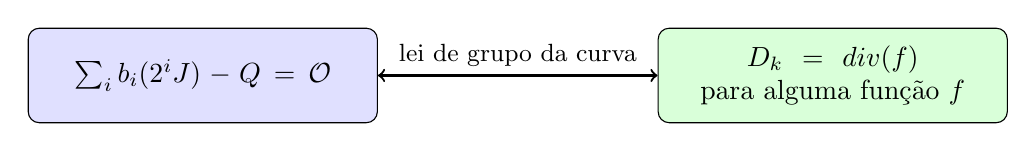
\begin{tikzpicture}[node distance=2cm]
 \tikzstyle{receipt}=[rectangle,rounded corners,draw=black,
   minimum width=4.4cm,minimum height=1.2cm,text centered,text width=4.2cm]
 \node (sum) [receipt,fill=blue!12]
   {\(\sum_i b_i(2^iJ)-Q=\mathcal O\)};
 \node (div) [receipt,right of=sum,xshift=6cm,fill=green!15]
   {\(D_k=\operatorname{div}(f)\)\\para alguma função \(f\)};
 \draw[<->,thick] (sum) --
   node[midway,above=2pt,font=\small,fill=white,inner sep=1pt]
   {lei de grupo da curva} (div);
\end{tikzpicture}
\end{center}

Não é necessário que a implementação use bits canónicos exactamente desta
maneira. O dispositivo actual admite representações escalares congruentes e
garante consistência da representação que reutiliza. O exemplo binário explicita o certificado; as condições exactas do circuito tratam a maleabilidade sem
pressupor que cada variável chamada \texttt{bit} foi automaticamente restringida a
\(0\) ou \(1\).

\subsection{Dois exemplos geométricos}
\label{sec:fcmp-divisor-pictures}

A equivalência \eqref{eq:fcmp-principal-divisor-criterion} já aparece em duas
funções conhecidas.

\subsubsection{A recta vertical}

Uma recta vertical passa por
\(P=(P_{\rm hor},P_{\rm ver})\), por
\(-P=(P_{\rm hor},-P_{\rm ver})\) e pelo ponto no infinito. Para um ponto
variável \(Q\), a função
\begin{align*}
 v_P(Q)=Q_{\rm hor}-P_{\rm hor}
\end{align*}
tem zeros em \(P\) e \(-P\) e um pólo duplo em \(\mathcal O\):
\begin{align}
 \operatorname{div}(v_P)
 =[P]+[-P]-2[\mathcal O].
 \label{eq:fcmp-vertical-divisor}
\end{align}
O grau é \(1+1-2=0\), e a soma de grupo é
\begin{align*}
 P+(-P)-2\mathcal O=\mathcal O.
\end{align*}
O divisor principal escreveu a lei do inverso.

\subsubsection{A recta por dois pontos}

Uma recta não vertical que passa por \(P\) e \(Q\) encontra a cúbica uma
terceira vez em \(-(P+Q)\). Chamando \(\mathcal L_{P,Q}\) à função dessa
recta,
\begin{align}
 \operatorname{div}(\mathcal L_{P,Q})
 =[P]+[Q]+[-(P+Q)]-3[\mathcal O].
 \label{eq:fcmp-line-divisor}
\end{align}
Outra vez,
\begin{align*}
 P+Q-(P+Q)=\mathcal O.
\end{align*}
O desenho usual da adição de pontos --- recta, terceira intersecção,
reflexão --- já era uma afirmação sobre um divisor principal. O método de
Eagen usa esta representação da lei de grupo por divisores.

\begin{center}
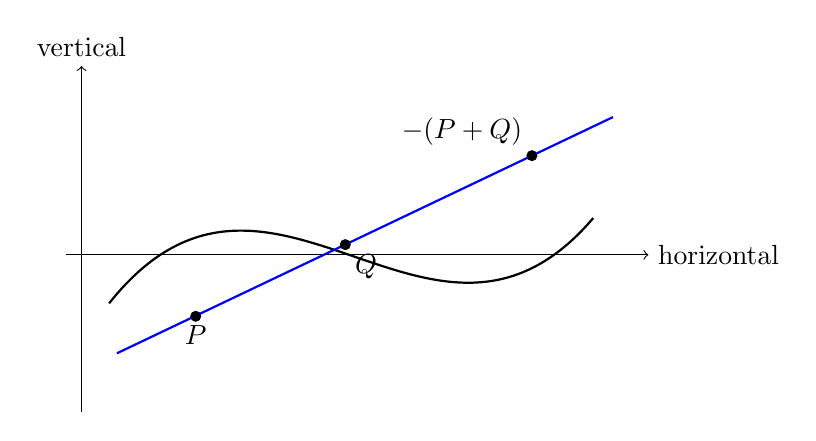
\begin{tikzpicture}[x=1cm,y=1cm]
 \draw[->] (-.2,0) -- (7.2,0) node[right]{horizontal};
 \draw[->] (0,-2.0) -- (0,2.4) node[above]{vertical};
 \draw[thick,domain=.35:6.5,samples=80,smooth]
   plot (\x,{.055*(\x-1.0)*(\x-3.4)*(\x-6.0)});
 \draw[thick,blue] (.45,-1.25) -- (6.75,1.75);
 \fill (1.45,-.78) circle (2pt) node[below]{\(P\)};
 \fill (3.35,.13) circle (2pt) node[below right]{\(Q\)};
 \fill (5.72,1.26) circle (2pt) node[above left]{\(-(P+Q)\)};
\end{tikzpicture}
\end{center}

No dispositivo real há muitas somas e multiplicidades, por isso a função
\(f(P)=A(P_{\rm hor})-P_{\rm ver}B(P_{\rm hor})\) é mais rica que uma recta.
A reciprocidade de Weil escolhe outra recta aleatória para auditar essa
função. Mas o certificado continua a dizer a mesma coisa que
\eqref{eq:fcmp-line-divisor}: os pontos listados fecham-se sob a lei de grupo.

\subsection{A função que testemunha o divisor}

Para um ponto \(P=(P_{\rm hor},P_{\rm ver})\) numa curva de Weierstrass
curta,
\begin{align*}
 P_{\rm ver}^{\,2}=P_{\rm hor}^{\,3}
   +a_{\rm curva}P_{\rm hor}+b_{\rm curva},
\end{align*}
uma função racional pode ser reduzida à forma
\begin{align}
 f(P)=A(P_{\rm hor})-P_{\rm ver}B(P_{\rm hor})
 \label{eq:fcmp-divisor-function-shape}
\end{align}
para polinómios \(A,B\) de graus limitados. Se
\(\operatorname{div}(f)=D_k\), os coeficientes de \(A\) e \(B\) são uma
testemunha algébrica de que os zeros e pólos alegados se equilibram.

Poderíamos pedir ao circuito que verificasse \(f\) em todos os pontos da
tabela. Isso voltaria a custar linearmente em todas as entradas, exactamente o
que queríamos evitar. Precisamos de testar a identidade sem avaliar separadamente todos os pontos.

\section{A linha aleatória e a troca de Weil}
\label{sec:fcmp-weil-reciprocity}

Escolha-se da transcrição uma linha de teste
\begin{align}
 \mathcal L_{\rm teste}(P)
   =P_{\rm ver}-c_{\rm declive}P_{\rm hor}-c_{\rm corte}.
 \label{eq:fcmp-random-line}
\end{align}
Uma linha encontra a curva elíptica em três pontos, contando
multiplicidades:
\begin{align*}
 P_{\rm linha,0},\ P_{\rm linha,1},\ P_{\rm linha,2},
 \qquad P_{\rm linha,0}+P_{\rm linha,1}+P_{\rm linha,2}=\mathcal O.
\end{align*}
O divisor da linha é, esquematicamente,
\begin{align*}
 \operatorname{div}(\mathcal L_{\rm teste})
  =[P_{\rm linha,0}]+[P_{\rm linha,1}]+[P_{\rm linha,2}]-3[\mathcal O].
\end{align*}

A reciprocidade de Weil diz, quando os suportes não colidem, que duas funções
racionais podem trocar o lugar onde são avaliadas:
\begin{align}
 f\bigl(\operatorname{div}\mathcal L_{\rm teste}\bigr)
   =\mathcal L_{\rm teste}\bigl(\operatorname{div}f\bigr).
 \label{eq:fcmp-weil-reciprocity}
\end{align}
Se
\begin{align*}
 f(D)=\prod_P f(P)^{m_P},
\end{align*}
então o lado esquerdo de \eqref{eq:fcmp-weil-reciprocity} avalia \(f\) apenas
nos três pontos aleatórios da linha. O lado direito avalia
\(\mathcal L_{\rm teste}\)
nos pontos que codificam a tabela de múltiplos e o resultado \(Q\). A
identidade substitui a avaliação de \(f\) em muitos pontos fixos pela avaliação
de \(f\) em três pontos aleatórios e de \(\mathcal L_{\rm teste}\) nos
pontos fixos.

\begin{center}
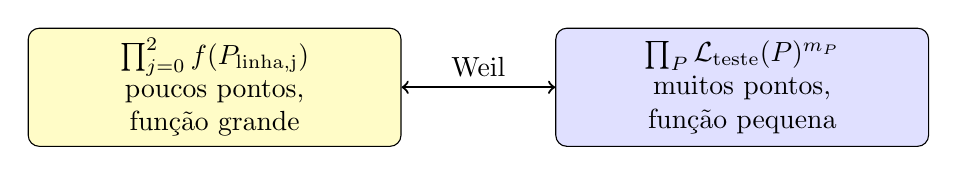
\begin{tikzpicture}[node distance=2cm]
 \tikzstyle{weilbox}=[rectangle,rounded corners,draw=black,
   minimum width=4.7cm,minimum height=1.5cm,text centered,text width=4.5cm]
 \node (left) [weilbox,fill=yellow!22]
   {\(\prod_{j=0}^{2}f(P_{\rm linha,j})\)\\poucos pontos, função grande};
 \node (right) [weilbox,right of=left,xshift=4.7cm,fill=blue!12]
   {\(\prod_P \mathcal L_{\rm teste}(P)^{m_P}\)\\
    muitos pontos, função pequena};
 \draw[<->,thick] (left) -- node[above]{Weil} (right);
\end{tikzpicture}
\end{center}

O desafio vem \emph{depois} de os compromissos à testemunha entrarem na
transcrição. O provador não pode escolher a função depois de ver uma linha
conveniente. Uma identidade racional falsa pode coincidir nos pontos
aleatórios por acaso, mas um polinómio não nulo de grau limitado tem apenas um
número limitado de raízes. Esta é uma aplicação do princípio de Schwartz--Zippel: avaliar num ponto aleatório transforma uma identidade inteira
num teste curto com erro desprezável.

\subsection{Produtos ainda são caros; deriva-se o logaritmo}

O lado
\begin{align*}
 \prod_P \mathcal L_{\rm teste}(P)^{m_P}
\end{align*}
contém produtos e expoentes dependentes da representação de \(k\). A derivada
logarítmica converte multiplicidades em coeficientes:
\begin{align}
 \mathrm d\log\left(\prod_i u_i^{m_i}\right)
   =\sum_i m_i\,\mathrm d\log u_i
   =\sum_i m_i\frac{\mathrm du_i}{u_i}.
 \label{eq:fcmp-logarithmic-derivative}
\end{align}
Em vez de construir uma sequência de produtos, o circuito verifica combinações
lineares de valores e inversos nos pontos desafiados. As inversões tornam-se
restrições multiplicativas
\begin{align*}
 u\cdot u^{-1}=1.
\end{align*}
O código amostra pontos de desafio na curva, calcula a linha que passa por
eles, avalia a testemunha do divisor e interpola a contribuição da tabela de
múltiplos. A igualdade final verifica que o certificado da soma escondida e o ponto
alegado produzem a mesma avaliação para a linha aleatória.

Não precisamos de copiar aqui as dezenas de coeficientes de \(A\),
\(B\), numeradores e denominadores. O que o leitor deve conseguir
reconstruir é a cadeia causal:
\begin{align*}
 Q=kJ
 &\Longrightarrow \sum_i b_i(2^iJ)-Q=\mathcal O\\
 &\Longrightarrow D_k\text{ é principal}\\
 &\Longrightarrow D_k=\operatorname{div}(f)\\
 &\Longrightarrow
 f(\operatorname{div}\mathcal L_{\rm teste})
   =\mathcal L_{\rm teste}(\operatorname{div}f)\\
 &\Longrightarrow
 \text{as avaliações comprimidas coincidem.}
\end{align*}
Na direcção de segurança, uma prova aceitável para uma igualdade falsa teria
de construir um divisor ou uma função inconsistente que sobrevivesse aos desafios
aleatórios e às restrições do argumento.

\subsection{Caso excepcional de normalização}

Fixar um coeficiente de \(f\) a \(1\) é uma forma de impedir a solução
inteiramente nula. Contudo, há divisores legítimos para os quais precisamente
esse coeficiente é zero. Uma revisão da zkSecurity chamou a atenção para esta
incompletude \cite{zksecurity-divisor-notes}. A consequência não é aceitar uma
prova falsa; é o provador, com probabilidade desprezável, escolher escalares de
ofuscação para os quais a forma normalizada não existe e não conseguir produzir
a prova.

Uma implementação robusta deve portanto:
\begin{align*}
 \text{amostrar os escalares de ofuscação}
 &\longrightarrow
 \text{construir e verificar que o divisor utilizável existe}\\
 &\longrightarrow \text{provar}.
\end{align*}
Se falhar, rejeitam-se esses escalares de ofuscação e reamostra-se. Na revisão
corrente de \texttt{monero-oxide}, o «x» do nome literal abaixo designa o
coeficiente do termo em x da função polinomial, não uma chave de gasto nem a
operação \(\operatorname{hor}(P)\); o fluxo é directamente
\begin{align*}
 \texttt{ScalarMulAndDivisor::new}
 &\longrightarrow \texttt{normalize\_x\_coefficient},\\
 \texttt{normalize\_x\_coefficient}
 &\longrightarrow \texttt{invert().unwrap()}.
\end{align*}
Não há ali verificação nem reamostragem \cite{monero-oxide-fcmp-source}. O
coeficiente zero excepcional provoca um \texttt{panic} no provador. Não se
fornece ao verificador uma inversão de zero e não se confunde uma falha rara de
completude com uma falha de solidez, mas o tratamento robusto dessa falha do
provador ainda falta nessa revisão.

\subsection{Interface abstracta do argumento}

Depois de abstrair o dispositivo, a demonstração usa a garantia seguinte:
se o verificador aceita, existe uma representação consistente de \(k\) tal
que \(Q=kJ\), salvo o erro associado ao desafio aleatório. Curve Trees usa
esta interface sem repetir a geometria algébrica em cada nível. A composição
de segurança enumera as instâncias, vincula as entradas e aplica a garantia a
cada uma.

\section{Tuplas de saída na instanciação do Monero}
\label{sec:fcmp-output-tuple}

Curve Trees acumula pontos genéricos. O Monero precisa de acumular os dados
necessários ao gasto de uma saída. Uma chave pública sozinha não chega:
temos de ligar a autorização, a imagem de chave que impedirá gasto duplo e o
compromisso de montante usado no equilíbrio. A folha FCMP++ é portanto a
tupla
\begin{align}
 \mathsf{Folha}=(O,I,C).
 \label{eq:fcmp-output-tuple}
\end{align}
Os três pontos têm funções diferentes:

\begin{description}
 \item[\(O\)] é a chave de saída, o ponto cuja abertura autoriza o gasto;
 \item[\(I\)] é a \emph{base} de imagem de chave derivada da chave de saída;
 não é ainda a imagem de chave publicada;
 \item[\(C\)] é o compromisso de montante associado à saída.
\end{description}

Nenhum destes pontos, isoladamente, é uma folha. A folha é sempre a tupla
ordenada \(\mathsf F_i=(O_i,I_i,C_i)\).

Os endereços de utilização única não desapareceram: em cada folha, \(O_i\) é
precisamente a chave pública de saída de utilização única. Para uma saída
histórica, \(k_{{\rm ligar},i}\) é a chave privada que a carteira recupera
para a gastar. FCMP++ não substitui essa derivação; substitui a lista explícita
usada para provar pertença.

Para uma saída histórica, escreva-se \(O_{\rm original}\) para a chave
publicada e \(O\) para o ponto, eventualmente limpo de torsão, inserido na
árvore. Então
\begin{align*}
 O=k_{\rm ligar}G,\qquad
 I=\mathcal H_p(O_{\rm original}),\qquad
 C=a_{\rm mont}G+v_{\rm mont}H,
\end{align*}
onde \(a_{\rm mont}\) é a máscara do compromisso e \(v_{\rm mont}\) o
montante. A construção do estado, não o circuito da prova, fixa \(I\) a partir
da codificação original. Aqui \(\mathcal H_p\) abrevia a variante definida
pelo formato: mapeamento enviesado para saídas legadas e não enviesado para
Carrot. A imagem de chave que aparecerá ao gastar é
\begin{align*}
 K_{\rm imagem}
   =k_{\rm ligar}I
   =k_{\rm ligar}\mathcal H_p(O_{\rm original}).
\end{align*}
Sem componente de torsão, \(O_{\rm original}=O\); a nota final explicita por
que a implementação conserva a distinção para saídas legadas. Esta regra de
construção da folha é parte da costura ponta a ponta: FCMP prova pertença do
\emph{mesmo} \(I\) que SAL usa, não volta a calculá-lo durante o gasto.

\subsection{Compatibilidade com formatos de chave futuros}

FCMP++ escreve a abertura geral de \(O\) como
\begin{align}
 O=k_{\rm ligar}G+k_{\rm autor}T.
 \label{eq:fcmp-output-general-opening}
\end{align}
As saídas antigas são representadas tomando \(k_{\rm autor}=0\). O gerador
\(T\) permite que um formato futuro use um segundo coeficiente de abertura sem
expulsar as saídas históricas da mesma árvore. Este coeficiente é um escalar
secreto; não é a coordenada vertical de \(O\).

Como o grupo é cíclico, existe matematicamente um logaritmo discreto que
relaciona \(T\) com \(G\). O protocolo exige que ninguém o conheça. Se essa
relação fosse conhecida, uma abertura poderia ser convertida noutra e o par
\((k_{\rm ligar},k_{\rm autor})\) deixaria de ser vinculante. Não daremos um
nome de uma só letra a um valor que não é testemunho e que ninguém deve
conhecer.

\section{Re-randomização da tupla de saída}
\label{sec:fcmp-output-rerandomization}

Não podemos revelar \((O,I,C)\) ao verificador da prova: ele procuraria a
tupla na árvore e descobriria imediatamente a folha. O provador escolhe novos
escalares de ofuscação
\begin{align*}
 m_O,\ m_I,\ m_{\rm esconder},\ m_C
   \quad\text{uniformes no campo escalar}
\end{align*}
e publica a tupla de entrada re-randomizada
\begin{align}
 \widetilde O&=O+m_OT,
 \label{eq:fcmp-rerand-o}\\
 \widetilde I&=I+m_IU,
 \label{eq:fcmp-rerand-i}\\
 R_{\rm ligar}&=m_IV+m_{\rm esconder}T,
 \label{eq:fcmp-rerand-r}\\
 \widetilde C&=C+m_CG.
 \label{eq:fcmp-rerand-c}
\end{align}

\begin{center}
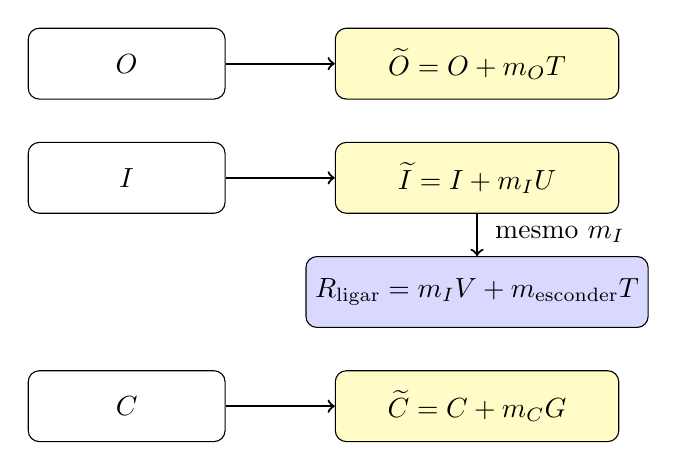
\begin{tikzpicture}[node distance=1.45cm]
 \tikzstyle{oldbox}=[rectangle,draw=black,rounded corners,
   minimum width=2.5cm,minimum height=.9cm,text centered]
 \tikzstyle{newbox}=[rectangle,draw=black,rounded corners,
   minimum width=3.6cm,minimum height=.9cm,text centered,fill=yellow!22]
 \node (o) [oldbox] {\(O\)};
 \node (ot) [newbox,right of=o,xshift=3.0cm]
   {\(\widetilde O=O+m_OT\)};
 \node (i) [oldbox,below of=o] {\(I\)};
 \node (it) [newbox,right of=i,xshift=3.0cm]
   {\(\widetilde I=I+m_IU\)};
 \node (rf) [newbox,below of=it,fill=blue!15]
   {\(R_{\rm ligar}=m_IV+m_{\rm esconder}T\)};
 \node (c) [oldbox,below of=i,yshift=-1.45cm] {\(C\)};
 \node (ct) [newbox,right of=c,xshift=3.0cm]
   {\(\widetilde C=C+m_CG\)};
 \draw[->,thick] (o) -- (ot);
 \draw[->,thick] (i) -- (it);
 \draw[->,thick] (c) -- (ct);
 \draw[->,thick] (it) -- node[right,xshift=1mm]{mesmo \(m_I\)} (rf);
\end{tikzpicture}
\end{center}

Cada base foi escolhida por uma razão:

\begin{itemize}
 \item somar \(m_OT\) transforma
 \(O=k_{\rm ligar}G+k_{\rm autor}T\) em
 \[
 \widetilde O=k_{\rm ligar}G+\widetilde k_{\rm autor}T,
 \qquad \widetilde k_{\rm autor}=k_{\rm autor}+m_O;
 \]
 o coeficiente de ligação \(k_{\rm ligar}\) fica intacto;
 \item somar \(m_IU\) esconde a base \(I\) da imagem de chave;
 \item \(R_{\rm ligar}\) compromete-se com o \emph{mesmo} \(m_I\) noutra base
 \(V\), enquanto \(m_{\rm esconder}T\) o oculta;
 \item somar \(m_CG\) muda apenas a máscara \(a_{\rm mont}\) do compromisso
 \(C=a_{\rm mont}G+v_{\rm mont}H\), conservando o montante
 \(v_{\rm mont}\).
\end{itemize}

Se usássemos apenas \(\widetilde I=I+m_IU\), a prova de autorização precisaria
de retirar \((k_{\rm ligar}m_I)U\) para recuperar
\(k_{\rm ligar}I\), mas não teria um compromisso público que vinculasse
\(m_I\) ao restante testemunho. \(R_{\rm ligar}\) fornece esse compromisso.
Ele não revela \(m_I\), porque está ofuscado pelo termo aleatório
\(m_{\rm esconder}T\), e não é o nonce da prova de Schnorr da raiz.

\subsection{O que o primeiro circuito verifica}

Dentro do primeiro circuito, o provador fornece aberturas que permitem recuperar
\((O,I,C)\) das versões públicas:
\begin{align*}
 O&=\widetilde O-m_OT,\\
 I&=\widetilde I-m_IU,\\
 C&=\widetilde C-m_CG.
\end{align*}
Também demonstra a decomposição
\begin{align*}
 R_{\rm ligar}=m_IV+m_{\rm esconder}T
\end{align*}
e, crucialmente, reutiliza \emph{as mesmas variáveis comprometidas} que
representam \(m_I\) na multiplicação por \(U\) e por \(V\). Não são duas
variáveis independentes com o mesmo nome; trata-se da mesma variável
comprometida no circuito.

Depois verifica que os três pontos recuperados estão na curva e comprime as
seis coordenadas
\begin{align}
 (O_{\rm hor},O_{\rm ver},I_{\rm hor},I_{\rm ver},
  C_{\rm hor},C_{\rm ver})
 \label{eq:fcmp-leaf-six-coordinates}
\end{align}
para testar que a tupla é uma das folhas do primeiro ramo. É por isso que a
folha tem seis escalares embora a vejamos como três pontos.

Nas camadas superiores, um nó já é o hash/compromisso de um ramo anterior. A
construção actual acumula a coordenada horizontal desse ponto no ramo seguinte e
usa o dispositivo por divisores para provar que a versão ofuscada abre para o
ponto válido correspondente. Assim, a primeira camada é especial:
\begin{align*}
 \text{folha}&:\quad 3\text{ pontos}=6\text{ coordenadas},\\
 \text{camada superior}&:\quad
   \text{coordenada horizontal do hash anterior}.
\end{align*}
As equações de curva e a prova de logaritmo discreto impedem que um rótulo
horizontal arbitrário seja aceite como o nó comprometido. As seis coordenadas
são as do modelo afim usado pelo circuito; não devem ser confundidas com os
bytes da codificação comprimida de Ed25519.

\section{A prova de pertença que resulta}
\label{sec:fcmp-membership-result}

Podemos agora escrever explicitamente a declaração FCMP. São públicos:

\begin{align*}
 &\mathcal R_{\rm tree},\\
 &(\widetilde O,\widetilde I,R_{\rm ligar},\widetilde C),\\
 &\text{o número e a forma das camadas},\\
 &\text{os parâmetros transparentes de Selene e Helios}.
\end{align*}

A testemunha contém:

\begin{align*}
 &(O,I,C),\quad m_O,m_I,m_{\rm esconder},m_C,\\
 &\text{a posição da tupla no primeiro ramo},\\
 &\text{os ramos e posições do caminho até à raiz},\\
 &\text{as aberturas dos compromissos vectoriais e testemunhas de divisores}.
\end{align*}

O verificador aprende apenas que existe uma testemunha que satisfaz:
\begin{enumerate}
 \item as quatro relações
 \eqref{eq:fcmp-rerand-o}--\eqref{eq:fcmp-rerand-c};
 \item que \((O,I,C)\) ocupa uma posição no primeiro ramo;
 \item que o hash de cada nó ocupa a posição vinculada no ramo seguinte;
 \item a ligação da raiz interna à raiz pública pela prova
 \eqref{eq:fcmp-root-pok-check}.
\end{enumerate}

O resultado ainda não demonstra que o provador conhece a abertura em
\(O=k_{\rm ligar}G+k_{\rm autor}T\), nem produz uma imagem de chave. Uma
pessoa que copiasse a tupla re-randomizada e a prova
de pertença não deveria por isso conseguir gastar. A prova de pertença demonstra que a entrada re-randomizada abre para uma saída
na árvore. A prova de autorização demonstra o conhecimento da abertura dessa
saída e deriva o marcador determinístico correspondente.

A separação permite usar uma prova especializada para comprimir a árvore e
outra para a autorização e a ligação.

\section{SAL: autorização de gasto e ligação}
\label{sec:fcmp-sal}

SAL abrevia \emph{Spend Authorization and Linkability}. Comecemos pelas
testemunhas conhecidas pelo provador:
\begin{align*}
 \widetilde O&=k_{\rm ligar}G+\widetilde k_{\rm autor}T,\\
 \widetilde I&=I+m_IU,\\
 R_{\rm ligar}&=m_IV+m_{\rm esconder}T.
\end{align*}
Queremos provar conhecimento da abertura
\((k_{\rm ligar},\widetilde k_{\rm autor})\), vincular a mesma máscara
\(m_I\) às duas provas e publicar
\begin{align}
 K_{\rm imagem}=k_{\rm ligar}I.
 \label{eq:fcmp-linking-tag-goal}
\end{align}

Para não carregar um produto anónimo chamado \(z\), damos-lhe o nome da sua
tarefa:
\begin{align*}
 p_{\rm cancelar}:=k_{\rm ligar}m_I.
\end{align*}
A relação que torna \(K_{\rm imagem}\) público sem revelar qual \(I\) estava
na árvore é
\begin{align}
 K_{\rm imagem}
   =k_{\rm ligar}\widetilde I-p_{\rm cancelar}U,
 \qquad p_{\rm cancelar}=k_{\rm ligar}m_I.
 \label{eq:fcmp-linking-tag-rerandomized}
\end{align}
Substituindo \(\widetilde I=I+m_IU\),
\begin{align*}
 K_{\rm imagem}
 &=k_{\rm ligar}(I+m_IU)-(k_{\rm ligar}m_I)U\\
 &=k_{\rm ligar}I+k_{\rm ligar}m_IU-k_{\rm ligar}m_IU\\
 &=k_{\rm ligar}I.
\end{align*}

\begin{center}
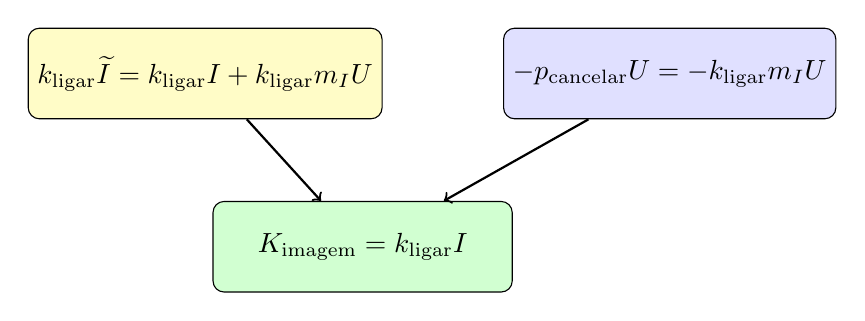
\begin{tikzpicture}[node distance=2cm]
 \tikzstyle{cancelbox}=[rectangle,rounded corners,draw=black,
   minimum width=3.8cm,minimum height=1.15cm,text centered]
 \node (masked) [cancelbox,fill=yellow!22]
   {\(k_{\rm ligar}\widetilde I
       =k_{\rm ligar}I+k_{\rm ligar}m_IU\)};
 \node (minus) [cancelbox,right of=masked,xshift=3.9cm,fill=blue!12]
   {\(-p_{\rm cancelar}U=-k_{\rm ligar}m_IU\)};
 \node (link) [cancelbox,below of=minus,xshift=-3.9cm,yshift=-.2cm,
   fill=green!18]
   {\(K_{\rm imagem}=k_{\rm ligar}I\)};
 \draw[->,thick] (masked) -- (link);
 \draw[->,thick] (minus) -- (link);
\end{tikzpicture}
\end{center}

O termo de ofuscação \(m_IU\) desaparece, mas só desaparece correctamente se o
mesmo \(m_I\) usado na prova de pertença entrar em
\(p_{\rm cancelar}=k_{\rm ligar}m_I\). É agora que \(R_{\rm ligar}\) passa a
ser usado na ligação entre as duas provas.

\subsection{Um compromisso que contém o produto}

SAL publica ainda
\begin{align}
 P_{\rm produto}
   =k_{\rm ligar}G+m_IV+p_{\rm cancelar}U+m_{\rm produto}T,
 \qquad p_{\rm cancelar}=k_{\rm ligar}m_I,
 \label{eq:fcmp-sal-p}
\end{align}
com uma nova máscara \(m_{\rm produto}\). \(P_{\rm produto}\) é um compromisso a
\((k_{\rm ligar},m_I,p_{\rm cancelar})\) nas bases \((G,V,U)\), escondido
com \(T\). Uma prova de estilo
Bulletproofs+ demonstra que a terceira coordenada é o produto das duas
primeiras:
\begin{align*}
 p_{\rm cancelar}=k_{\rm ligar}m_I.
\end{align*}

Contudo, \(P_{\rm produto}\) sozinho ainda poderia conter valores sem relação com
\(\widetilde O\), \(R_{\rm ligar}\) ou \(K_{\rm imagem}\). Três provas Schnorr generalizadas
partilham respostas com a prova do produto:

\begin{align}
 \widetilde O&=k_{\rm ligar}G+\widetilde k_{\rm autor}T,
 \label{eq:fcmp-sal-open-o}\\
 P_{\rm produto}-\widetilde O-R_{\rm ligar}
   &=p_{\rm cancelar}U+m_{\rm resto}T,
 \label{eq:fcmp-sal-open-p-prime}\\
 K_{\rm imagem}
   &=k_{\rm ligar}\widetilde I-p_{\rm cancelar}U,
 \label{eq:fcmp-sal-open-l}
\end{align}
onde
\begin{align*}
 m_{\rm resto}=m_{\rm produto}-\widetilde k_{\rm autor}-m_{\rm esconder}.
\end{align*}

A segunda igualdade expande-se como segue:
\begin{align*}
 P_{\rm produto}-\widetilde O-R_{\rm ligar}
 &=(k_{\rm ligar}G+m_IV+p_{\rm cancelar}U+m_{\rm produto}T)\\
 &\quad-(k_{\rm ligar}G+\widetilde k_{\rm autor}T)
       -(m_IV+m_{\rm esconder}T)\\
 &=p_{\rm cancelar}U
   +(m_{\rm produto}-\widetilde k_{\rm autor}-m_{\rm esconder})T\\
 &=p_{\rm cancelar}U+m_{\rm resto}T.
\end{align*}
Os termos em \(G\) e \(V\) cancelam. Portanto, o \(m_I\) comprometido em
\(P_{\rm produto}\) tem de ser compatível com o \(m_IV\) de
\(R_{\rm ligar}\), enquanto \eqref{eq:fcmp-sal-open-l} liga
\(k_{\rm ligar}\) e \(p_{\rm cancelar}\) à imagem de chave.

\section{As quatro equações do verificador SAL}
\label{sec:fcmp-sal-verifier}

Escrevemos agora as equações completas, mas sem baptizar segredos com um
alfabeto à parte. Denotemos por \(\mathbb F_{\rm esc}\) o campo escalar do
grupo. Além de \(m_{\rm produto}\), já escolhido, o provador usa sete nonces
aleatórios,
cada qual com o nome daquilo que irá esconder:
\begin{align*}
 n_{\rm ligar},n_I,n_{T,{\rm linear}},n_{T,{\rm constante}},
 n_{\rm autor},n_{\rm produto},n_{\rm resto}
   \in_R\mathbb F_{\rm esc}.
\end{align*}
Com eles constrói cinco pontos:
\begin{align}
 A_{\rm produto}
 &=n_{\rm ligar}G+n_IV+
   (n_{\rm ligar}m_I+n_Ik_{\rm ligar})U+n_{T,{\rm linear}}T,
 \label{eq:fcmp-sal-a}\\
 B_{\rm produto}&=n_{\rm ligar}n_IU+n_{T,{\rm constante}}T,
 \label{eq:fcmp-sal-b}\\
 N_O&=n_{\rm ligar}G+n_{\rm autor}T,
 \label{eq:fcmp-sal-ro}\\
 N_P&=n_{\rm produto}U+n_{\rm resto}T,
 \label{eq:fcmp-sal-rp}\\
 N_K&=n_{\rm ligar}\widetilde I-n_{\rm produto}U.
 \label{eq:fcmp-sal-rl}
\end{align}
Na implementação, \(\mathcal H_{\rm esc}\) reduz a um escalar uma saída BLAKE2b de 64
bytes, com a personalização \texttt{Monero}. Chamemos
\(c_{\rm SAL}\) ao desafio:
\begin{align*}
 c_{\rm SAL}=\mathcal H_{\rm esc}(&\text{hash da transacção},
 \widetilde O,\widetilde I,\widetilde C,R_{\rm ligar},\\
 &K_{\rm imagem},P_{\rm produto},A_{\rm produto},B_{\rm produto},
 N_O,N_P,N_K).
\end{align*}
Assim a transcrição prende a prova à transacção e a todos os pontos que as
quatro linhas seguintes irão relacionar. Para não tornar cada equação
ilegível, escrevemos apenas \(c=c_{\rm SAL}\) daqui até ao fim da derivação.
As respostas são
\begin{align}
 s_{\rm ligar}&=n_{\rm ligar}+c k_{\rm ligar},
 &s_I&=n_I+c m_I,
 \label{eq:fcmp-sal-responses-one}\\
 s_T&=n_{T,{\rm constante}}+c n_{T,{\rm linear}}+c^2m_{\rm produto},
 &s_{\rm autor}&=n_{\rm autor}+c\widetilde k_{\rm autor},
 \label{eq:fcmp-sal-responses-two}\\
 s_{\rm produto}&=n_{\rm produto}+c p_{\rm cancelar},
 &s_{\rm resto}&=n_{\rm resto}+c m_{\rm resto}.
 \label{eq:fcmp-sal-responses-three}
\end{align}

O verificador aceita as quatro relações:
\begin{align}
 c^2P_{\rm produto}+cA_{\rm produto}+B_{\rm produto}
 &=cs_{\rm ligar}G+cs_IV+s_{\rm ligar}s_IU+s_TT,
 \label{eq:fcmp-sal-verify-bp}\\
 N_O+c\widetilde O
 &=s_{\rm ligar}G+s_{\rm autor}T,
 \label{eq:fcmp-sal-verify-o}\\
 N_P+c(P_{\rm produto}-\widetilde O-R_{\rm ligar})
 &=s_{\rm produto}U+s_{\rm resto}T,
 \label{eq:fcmp-sal-verify-p}\\
 N_K+cK_{\rm imagem}
 &=s_{\rm ligar}\widetilde I-s_{\rm produto}U.
 \label{eq:fcmp-sal-verify-l}
\end{align}

As quatro equações parecem fechaduras diferentes, mas usam as mesmas chaves
algébricas \(s_{\rm ligar}\) e \(s_{\rm produto}\). Essa reutilização e o
mesmo \(R_{\rm ligar}\) público impedem misturar a pertença de uma saída com
a autorização de outra. Verifiquemos linha por linha.

\subsection{Primeira linha: verificar o produto que cancela a máscara}

Expanda o lado direito de \eqref{eq:fcmp-sal-verify-bp}:
\begin{align*}
 &c(n_{\rm ligar}+ck_{\rm ligar})G
   +c(n_I+cm_I)V\\
 &\quad +(n_{\rm ligar}+ck_{\rm ligar})(n_I+cm_I)U
   +(n_{T,{\rm constante}}+cn_{T,{\rm linear}}+c^2m_{\rm produto})T\\
 &=cn_{\rm ligar}G+c^2k_{\rm ligar}G
   +cn_IV+c^2m_IV\\
 &\quad+\bigl(n_{\rm ligar}n_I
   +cn_{\rm ligar}m_I+cn_Ik_{\rm ligar}
   +c^2k_{\rm ligar}m_I\bigr)U\\
 &\quad+n_{T,{\rm constante}}T+cn_{T,{\rm linear}}T
   +c^2m_{\rm produto}T.
\end{align*}
Agrupando por potências de \(c\), obtemos
\begin{align*}
 &=\underbrace{n_{\rm ligar}n_IU+n_{T,{\rm constante}}T}_{B_{\rm produto}}\\
 &\quad+c\underbrace{\bigl(n_{\rm ligar}G+n_IV
   +(n_{\rm ligar}m_I+n_Ik_{\rm ligar})U
   +n_{T,{\rm linear}}T\bigr)}_{A_{\rm produto}}\\
 &\quad+c^2\underbrace{\bigl(k_{\rm ligar}G+m_IV
   +k_{\rm ligar}m_IU+m_{\rm produto}T\bigr)}_{P_{\rm produto}}.
\end{align*}
É exactamente o lado esquerdo porque
\(p_{\rm cancelar}=k_{\rm ligar}m_I\). O produto das duas respostas cria ao
mesmo tempo os termos lineares de \(A_{\rm produto}\) e o produto verdadeiro
de \(P_{\rm produto}\). Esta é a pequena engrenagem Bulletproofs+ dentro da
SAL.

\subsection{Segunda linha: a mesma chave abre a saída}

Usando
\(\widetilde O=k_{\rm ligar}G+\widetilde k_{\rm autor}T\),
\begin{align*}
 N_O+c\widetilde O
 &=n_{\rm ligar}G+n_{\rm autor}T
   +c(k_{\rm ligar}G+\widetilde k_{\rm autor}T)\\
 &=(n_{\rm ligar}+ck_{\rm ligar})G
   +(n_{\rm autor}+c\widetilde k_{\rm autor})T\\
 &=s_{\rm ligar}G+s_{\rm autor}T.
\end{align*}
Não aparece uma segunda resposta para a chave. Reutiliza-se
\(s_{\rm ligar}\); logo o \(k_{\rm ligar}\) comprometido em
\(P_{\rm produto}\) é precisamente o que abre \(\widetilde O\).

\subsection{Terceira linha: a máscara é a mesma da FCMP}

Da equação \eqref{eq:fcmp-sal-open-p-prime},
\begin{align*}
 N_P+c(P_{\rm produto}-\widetilde O-R_{\rm ligar})
 &=n_{\rm produto}U+n_{\rm resto}T
   +c(p_{\rm cancelar}U+m_{\rm resto}T)\\
 &=(n_{\rm produto}+cp_{\rm cancelar})U
   +(n_{\rm resto}+cm_{\rm resto})T\\
 &=s_{\rm produto}U+s_{\rm resto}T.
\end{align*}
Aqui a resposta partilhada é \(s_{\rm produto}\). Portanto o produto da
primeira linha é o mesmo valor que sobra depois de subtrair
\(\widetilde O\) e \(R_{\rm ligar}\) a \(P_{\rm produto}\). A SAL não pode
trocar silenciosamente o \(m_I\) que a FCMP usou para ofuscar \(I\).

\subsection{Quarta linha: a imagem de chave fica determinística}

Finalmente, usando
\(K_{\rm imagem}=k_{\rm ligar}\widetilde I-p_{\rm cancelar}U\),
\begin{align*}
 N_K+cK_{\rm imagem}
 &=n_{\rm ligar}\widetilde I-n_{\rm produto}U
   +c(k_{\rm ligar}\widetilde I-p_{\rm cancelar}U)\\
 &=(n_{\rm ligar}+ck_{\rm ligar})\widetilde I
   -(n_{\rm produto}+cp_{\rm cancelar})U\\
 &=s_{\rm ligar}\widetilde I-s_{\rm produto}U.
\end{align*}
Esta linha reutiliza ambas as respostas decisivas. Assim não basta abrir
\(\widetilde O\), construir outro produto e inventar uma imagem de chave
independente: depois de sair o desafio, todos têm de contar a mesma história.

\subsection{Derivação da ligação}

Uma saída concreta traz um ponto \(I\) fixo no estado da cadeia e um
coeficiente de ligação \(k_{\rm ligar}\) fixo na abertura autorizada. Em
particular, a integração constrói \(I\) a partir da codificação pública
original da saída; o circuito FCMP recebe-o como parte da folha, não o
recalcula. Qualquer gasto honesto produz
\begin{align*}
 K_{\rm imagem}=k_{\rm ligar}I,
\end{align*}
independentemente das novas máscaras
\(m_O,m_I,m_{\rm esconder},m_C,m_{\rm produto}\). Duas tentativas de gastar a
mesma
saída publicam o mesmo \(K_{\rm imagem}\), e os nós rejeitam a repetição.
Saídas diferentes deverão produzir marcadores não relacionados.

O verificador nunca recebe \(I\) em claro. Recebe \(\widetilde I\), que muda
a cada re-randomização, e \(K_{\rm imagem}\), que é determinístico. A SAL
prova que a máscara foi cancelada de modo consistente, sem revelar de que
folha veio o ponto. É a propriedade de ligação que antes vinha da imagem de
chave CLSAG; a lista explícita do anel foi substituída por uma prova de
pertença separada.

\section{Composição completa}
\label{sec:fcmp-full-composition}

O protocolo pode agora ser percorrido da esquerda para a direita sem saltar a
costura entre pertença e autorização:

\begin{center}
\begin{tikzpicture}
 \tikzstyle{flowbox}=[rectangle,rounded corners,draw=black,
   minimum width=6.0cm,minimum height=.75cm,text centered,text width=5.7cm,
   inner sep=2pt,font=\small]
 \node (chain) [flowbox,fill=green!17]
   {cadeia: folha \((O,I,C)\)};
 \node (rerand) [flowbox,below=.12cm of chain,fill=yellow!22]
   {re-randomizar: \((\widetilde O,\widetilde I,R_{\rm ligar},\widetilde C)\)};
 \node (member) [flowbox,below=.12cm of rerand,xshift=-3.15cm,
   minimum height=1.05cm,fill=blue!12]
   {FCMP: abrir a tupla\\e subir até
   \(\mathcal R_{\rm tree}\)};
 \node (sal) [flowbox,below=.12cm of rerand,xshift=3.15cm,
   minimum height=1.05cm,fill=blue!12]
   {SAL: abrir \(\widetilde O\); cancelar \(m_I\)\\
   e vincular \(K_{\rm imagem}\)};
 \node (tx) [flowbox,below=.12cm of sal,xshift=-3.15cm,
   minimum width=9.0cm,text width=8.7cm,fill=green!17]
   {transacção aceite: pertença + autorização\\
   + equilíbrio + imagem de chave nova};
 \draw[->,thick] (chain) -- (rerand);
 \draw[->,thick] (rerand) -- (member);
 \draw[->,thick] (rerand) -- (sal);
 \draw[->,thick] (member) -- (tx);
 \draw[->,thick] (sal) -- (tx);
\end{tikzpicture}
\end{center}

A bifurcação é literal: a FCMP prova pertença e a SAL prova autorização. A
tupla pública idêntica com \(R_{\rm ligar}\) une os ramos; só a junção conclui
\(K_{\rm imagem}=k_{\rm ligar}I\): a folha é real e Alice pode gastá-la.

Os dados públicos relevantes para esta costura são:
\begin{align*}
 \mathsf{Prova}_{\rm FCMP}
   &\longleftrightarrow
   (\widetilde O,\widetilde I,R_{\rm ligar},\widetilde C,
     \mathcal R_{\rm tree}),\\
 \mathsf{Prova}_{\rm SAL}
   &\longleftrightarrow
   (\widetilde O,\widetilde I,R_{\rm ligar},\widetilde C,K_{\rm imagem},
     \mathcal H(\text{transacção})).
\end{align*}
\(\widetilde C\) entra na transcrição SAL embora as equações
\eqref{eq:fcmp-sal-verify-bp}--\eqref{eq:fcmp-sal-verify-l} não o abram:
FCMP liga-o ao compromisso histórico e as regras RingCT ligam os
pseudo-compromissos ao equilíbrio da transacção. O hash comum impede reutilizar
a SAL numa transacção diferente.

\subsection{Ordem de verificação}

Se preferir verificar de trás para a frente:

\begin{enumerate}
 \item \(K_{\rm imagem}\) ainda não apareceu antes; logo não é um gasto
 duplo conhecido.
 \item A SAL prova conhecimento de
 \(k_{\rm ligar},\widetilde k_{\rm autor},m_I,m_{\rm esconder},
 m_{\rm produto}\), com
 \(p_{\rm cancelar}=k_{\rm ligar}m_I\), compatíveis com
 \(\widetilde O,\widetilde I,R_{\rm ligar}\), e impõe
 \(K_{\rm imagem}=k_{\rm ligar}\widetilde I-p_{\rm cancelar}U\).
 \item A FCMP prova que esses mesmos pontos re-randomizados abrem para uma
 tupla \((O,I,C)\) numa folha, em particular
 \(\widetilde I=I+m_IU\). Só a composição permite concluir
 \(K_{\rm imagem}=k_{\rm ligar}I\).
 \item O caminho Curve Trees termina numa raiz interna que satisfaz
 \(\widehat{\mathcal R}-\mathcal R_{\rm tree}
   =m_{\rm raiz}H_{\rm raiz}\), para uma
 máscara de raiz \(m_{\rm raiz}\) conhecida pelo provador.
 \item A raiz pública compromete o conjunto de saídas admissíveis naquele
 estado da cadeia.
\end{enumerate}

Nenhum passo isolado prova todas as propriedades. A segurança da composição
depende de as variáveis de saída de cada passo serem as variáveis de entrada
do passo seguinte.

\section{Um exemplo pequeno de ponta a ponta}
\label{sec:fcmp-end-to-end-toy}

Façamos uma execução conceptual com números simbólicos. A árvore contém quatro
folhas:
\begin{align*}
 (O_0,I_0,C_0),\ldots,(O_3,I_3,C_3).
\end{align*}
O provador possui a terceira, índice secreto \(2\). Chamemos
\(O_{2,{\rm original}}\) à codificação pública original e \(O_2\) ao ponto
inserido na árvore. Então
\begin{align*}
 O_2&=k_{\rm ligar}G+k_{\rm autor}T,\\
 I_2&=\mathcal H_p(O_{2,{\rm original}}),\\
 C_2&=a_{\rm montante}G+v_{\rm montante}H.
\end{align*}
Escolhe máscaras novas e anuncia
\begin{align*}
 \widetilde O&=O_2+m_OT,\\
 \widetilde I&=I_2+m_IU,\\
 R_{\rm ligar}&=m_IV+m_{\rm esconder}T,\\
 \widetilde C&=C_2+m_CG.
\end{align*}

O primeiro circuito recupera os três pontos sem os publicar, agrega as seis
coordenadas com seis pesos derivados da transcrição e obtém
\begin{align*}
 v_{\rm alvo}
 &=w_{O,{\rm hor}}O^{\rm hor}_2+w_{O,{\rm ver}}O^{\rm ver}_2
   +w_{I,{\rm hor}}I^{\rm hor}_2+w_{I,{\rm ver}}I^{\rm ver}_2\\
 &\quad+w_{C,{\rm hor}}C^{\rm hor}_2+w_{C,{\rm ver}}C^{\rm ver}_2.
\end{align*}
Para cada folha \(j\), calcula dentro dos compromissos o agregado
\begin{align*}
 v_j=w_{O,{\rm hor}}O^{\rm hor}_j+w_{O,{\rm ver}}O^{\rm ver}_j
     +\cdots+w_{C,{\rm ver}}C^{\rm ver}_j
\end{align*}
e impõe
\begin{align*}
 (v_0-v_{\rm alvo})(v_1-v_{\rm alvo})
 (v_2-v_{\rm alvo})(v_3-v_{\rm alvo})=0.
\end{align*}
O factor \(v_2-v_{\rm alvo}\) é zero. O verificador não sabe qual factor.

Se houvesse mais níveis, o circuito abriria o compromisso deste ramo,
re-randomizaria o nó resultante e repetiria a selecção no pai, alternando
Selene e Helios, até obter \(\widehat{\mathcal R}\). A prova Schnorr autentica
\begin{align*}
 \widehat{\mathcal R}-\mathcal R_{\rm tree}=m_{\rm raiz}H_{\rm raiz}.
\end{align*}

Em paralelo, o provador calcula
\begin{align*}
 p_{\rm cancelar}&=k_{\rm ligar}m_I,\\
 K_{\rm imagem}
   &=k_{\rm ligar}\widetilde I-p_{\rm cancelar}U
     =k_{\rm ligar}I_2
\end{align*}
e produz a SAL. Se tentar gastar a mesma folha amanhã com escalares de
ofuscação totalmente novos, FCMP e SAL terão outra aparência, mas
\begin{align*}
 K'_{\rm imagem}=k_{\rm ligar}I_2=K_{\rm imagem}.
\end{align*}
O caminho não denuncia a posição; o marcador denuncia a repetição. Essa
assimetria é o objectivo inteiro.

\subsection{O que um observador consegue comparar}

Entre dois gastos distintos, o observador vê:
\begin{align*}
 &\widetilde O,\widetilde I,R_{\rm ligar},\widetilde C,
 P_{\rm produto},A_{\rm produto},B_{\rm produto},
 N_O,N_P,N_K,\text{ respostas},K_{\rm imagem}.
\end{align*}
Todos os pontos excepto \(K_{\rm imagem}\) incorporam nonces ou máscaras
novas,
directa ou indirectamente. A transcrição liga-os à transacção. Para a mesma saída,
\(K_{\rm imagem}\) repete-se e o segundo gasto é inválido. Para saídas diferentes, não há
um teste público que compare as respectivas folhas na árvore.

Uma prova de conhecimento zero formal precisa demonstrar esta
indistinguibilidade por simuladores e jogos, não apenas pela contagem de
termos aleatórios. A contagem identifica quais pontos devem ser re-randomizados e qual marcador
deve permanecer determinístico.

\section{Famílias de logaritmos desconhecidos}
\label{sec:fcmp-unknown-dlogs}

No compromisso de montante já usávamos duas bases, \(G\) e \(H\), sem que
ninguém devesse conhecer o escalar que transforma uma na outra. FCMP++ usa
uma família maior. No grupo da saída aparecem
\begin{align*}
 G,\ H,\ T,\ U,\ V,\ I.
\end{align*}
Nas curvas Selene e Helios aparecem ainda
\begin{align*}
 g,\ h,\ \mathbf g,\ \mathbf h,\ J_{\rm init}.
\end{align*}

Então FCMP++ trouxe três novos \(H\)? Trouxe três bases independentes para
papéis novos, não três cópias funcionais do compromisso de montante. Como o
grupo é cíclico, cada uma é algum múltiplo de \(G\); a segurança exige que
ninguém conheça esses multiplicadores nem uma relação linear útil entre as
bases. Não precisamos de dar nomes a números que ninguém conhece. Precisamos
de saber onde cada ponto trabalha:

\begin{center}
\renewcommand{\arraystretch}{1.25}
\begin{tabular}{|c|c|c|}
 \hline
 \textbf{base} & \textbf{onde trabalha} & \textbf{relação desconhecida}\\
 \hline
 \(H\) & \(C=a_{\rm montante}G+v_{\rm montante}H\), montante &
 relação entre \(G\) e \(H\)\\
 \hline
 \(T\) & \(O=k_{\rm ligar}G+k_{\rm autor}T\), segunda base da abertura &
 relação entre \(G\) e \(T\)\\
 \hline
 \(U\) & \(\widetilde I-I=m_IU\), máscara de \(I\) &
 relação entre \(G\) e \(U\)\\
 \hline
 \(V\) & \(R_{\rm ligar}=m_IV+m_{\rm esconder}T\), compromisso a \(m_I\) &
 relações entre \(G,T,V\)\\
 \hline
\end{tabular}
\end{center}

Precisão: \(I\) muda com a saída. As bases dos Bulletproofs são uma família
estática e indexada, não um único ponto nomeado. \(H\) é a base histórica de
montante; FCMP++ acrescenta \(T,U,V\) como bases globais com outras funções.

Como a SAL mistura \(G,T,U,V\), a hipótese útil é conjunta: um adversário não
deve conseguir encontrar
\begin{align}
 q_GG+q_TT+q_UU+q_VV=\mathcal O
 \label{eq:fcmp-output-generators-relation}
\end{align}
com pelo menos um dos coeficientes \(q_G,q_T,q_U,q_V\) diferente de zero.
Conhecer, por exemplo, a relação escalar entre \(T\) e \(V\) já daria uma
igualdade destas. Por isso a hipótese adequada é
\emph{logaritmo discreto generalizado}, não uma colecção de «segredos
mestres». \(T,U,V\)
são derivados por hash para ponto, com rótulos distintos e reproduzíveis;
\(G\) é canónico e \(H\) conserva a derivação histórica.

\subsection{Relação desconhecida não é testemunho desconhecido}

Há três situações que convém não misturar:

\begin{enumerate}
 \item a relação entre \(T\) e \(G\), desconhecida por todos: bases de um
 compromisso;
 \item \(O=k_{\rm ligar}G\), com \(k_{\rm ligar}\) conhecido pelo provador:
 uma chave pública;
 \item \(O=k_{\rm ligar}G\) e
 \(K_{\rm imagem}=k_{\rm ligar}I\): o mesmo testemunho conhecido em duas
 bases cuja relação é desconhecida.
\end{enumerate}

O dispositivo por divisores prepara deliberadamente
\begin{align*}
 J,\ 2J,\ 4J,\ldots,2^{n-1}J.
\end{align*}
Essas relações são públicas por desenho; não são parâmetros comprometidos. O
dispositivo prova que uma representação escondida selecciona e soma estes
múltiplos de modo consistente. A simples detecção de qualquer igualdade
entre pontos marcaria como «suspeita» precisamente a tabela que o algoritmo
precisa.

\subsection{Se uma relação multibase fosse conhecida}

Suponha-se que alguém conhece
\begin{align*}
 q_GG+q_TT+q_UU+q_VV=\mathcal O
\end{align*}
com, digamos, \(q_V\ne0\). Então pode isolar
\begin{align*}
 V=-q_V^{-1}(q_GG+q_TT+q_UU).
\end{align*}
Um compromisso que usava \(V\) como coordenada independente passa a poder ser
reescrito nas outras três bases. Dependendo dos coeficientes, isto pode criar
aberturas alternativas para \(P_{\rm produto}\) ou \(R_{\rm ligar}\) e destruir o argumento
de que as respostas partilhadas representam testemunhos únicos.

Não afirmamos que qualquer relação dê automaticamente a mesma exploração que
uma relação entre \(G\) e \(H\) daria aos montantes; é preciso seguir onde as
bases entram. A regra de auditoria é mais precisa: toda redução que usa vinculação de um
compromisso multibase deve enumerar a família de geradores e a hipótese de
relações lineares, em vez de afirmar apenas «assumimos o PLD».

\section{Actualização incremental da Curve Tree}
\label{sec:fcmp-tree-growth}

Enquanto se acrescentam saídas a uma dada versão da cadeia, a Curve Tree cresce
incrementalmente. Enquanto um ramo ainda tem lugares vazios, o acumulador pode
representá-los por escalares zero.
Se o lugar \(j\) tinha o valor \(v_j\) e recebe \(v_j'\), o compromisso muda
por
\begin{align}
 P_{\rm novo}=P_{\rm antigo}+(v_j'-v_j)G_j.
 \label{eq:fcmp-hash-grow}
\end{align}
Não é preciso recomputar as restantes multiplicações. O hash de um ramo
parcial já ocupa uma posição no pai e muda enquanto chegam filhos. Quando o
ramo enche, esse hash congela na posição; a folha seguinte abre um ramo irmão.
Se o pai já não tiver lugar, o transporte continua para cima, como numa soma
posicional.

\begin{center}
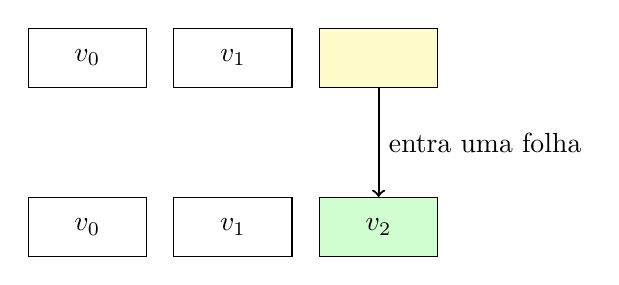
\begin{tikzpicture}[node distance=1.6cm]
 \tikzstyle{slot}=[rectangle,draw=black,minimum width=1.5cm,
   minimum height=.75cm,text centered]
 \node (a0) [slot] {\(v_0\)};
 \node (a1) [slot,right of=a0,xshift=.25cm] {\(v_1\)};
 \node (a2) [slot,right of=a1,xshift=.25cm,fill=yellow!20] {\(\square\)};
 \node (b0) [slot,below of=a0,yshift=-.55cm] {\(v_0\)};
 \node (b1) [slot,right of=b0,xshift=.25cm] {\(v_1\)};
 \node (b2) [slot,right of=b1,xshift=.25cm,fill=green!18] {\(v_2\)};
 \draw[->,thick] (a2) -- node[right]{entra uma folha} (b2);
\end{tikzpicture}
\end{center}

O \(\square\) é codificado internamente por zeros de enchimento. Na primeira
camada, uma folha válida exige duas coordenadas para cada ponto não identidade
\((O,I,C)\), todos verificados na curva; zeros de enchimento não formam tal
tupla. Nas camadas seguintes, o teste usa o ramo já preenchido até ao tamanho
esperado. O enchimento é aritmética do compromisso, não uma nova saída
gastável.

Uma nova folha altera todos os nós no seu caminho até ao topo, logo altera a
raiz. Isto não invalida a matemática de raízes antigas: cada raiz continua a
comprometer o seu instantâneo da árvore. A regra de consenso que decide qual
raiz uma transacção pode referir e por quanto tempo é uma política de
implantação por cima do acumulador. A prova recebe uma raiz concreta como
parte da declaração; não prova, por si só, que a raiz satisfaz uma política temporal de
actualidade.

\subsection{Por que as camadas superiores guardam só a coordenada horizontal}

Uma folha precisa de \(O,I,C\) completos porque essas identidades serão
abertas e usadas no gasto. Um nó superior só precisa de um rótulo vinculante
para o hash do ramo inferior. A construção usa directamente
\(\operatorname{hor}(P_j)\) como rótulo e compromete-o no pai. No exemplo
ternário, esses mesmos
rótulos foram escritos
\(P_j^{\rm hor}=\operatorname{hor}(P_j)\) e
\(Q_k^{\rm hor}=\operatorname{hor}(Q_k)\). Assim,
cada filho ocupa uma posição escalar, em vez de duas coordenadas.

Uma mesma coordenada horizontal pode corresponder a \(P\) e \(-P\). A árvore
superior é deliberadamente definida sobre o rótulo
\(\operatorname{hor}(P)\), não sobre uma codificação afim injectiva. O
circuito não recebe, contudo, um sinal à escolha sem
consequências: demonstra que o ponto ofuscado abre para um ponto válido e que
esse ponto é o compromisso/hash construído pelo ramo anterior. A pertença no
pai verifica somente se a sua coordenada horizontal está na lista, que é a relação
especificada. A especificação deve, por isso, tratar explicitamente esta identificação
entre \(P\) e \(-P\).

\section{O que mudou relativamente à CLSAG}
\label{sec:fcmp-versus-clsag}

A CLSAG reúne, num percurso circular, a escolha entre membros explícitos, o
conhecimento das chaves e a imagem de chave. FCMP++ separa três componentes:

\begin{description}
 \item[conjunto:] uma raiz pública compromete a árvore; os membros não são
 copiados para a transacção;
 \item[pertença:] Generalized Bulletproofs prova um caminho de uma tupla
 re-randomizada à raiz;
 \item[autorização e ligação:] SAL prova a abertura da chave e produz
 \(K_{\rm imagem}\).
\end{description}

Na CLSAG, aumentar o anel aumenta a lista de chaves e compromissos que a
transacção referencia. Em Curve Trees, aumentar o conjunto enche ramos e só
ocasionalmente acrescenta uma camada. O custo por prova depende do número de
camadas e das capacidades dos ramos, não é uma linha por saída histórica.

Também muda quem escolhe o conjunto. Uma carteira CLSAG selecciona desvios e
essa selecção pode introduzir distribuições reconhecíveis. Uma FCMP refere um
estado canónico do acumulador. «Cadeia completa» não quer dizer literalmente
qualquer byte que já apareceu: só entram tuplas que as regras consideram
saídas admissíveis, com validação de pontos e tratamento de compatibilidade.
A carteira deixa de seleccionar um pequeno conjunto de desvios segundo uma
distribuição própria.

\subsection{Análise de quatro tentativas de falsificação}

Podemos testar as fronteiras tentando fazer batota:

\begin{enumerate}
 \item \textbf{Inventar uma folha e conhecer o factor de ofuscação da raiz.}
 A prova Schnorr passa apenas se a raiz interna diferir da pública por
 \(m_{\rm raiz}H_{\rm raiz}\); o circuito de pertença continua a ter de abrir um caminho
 válido.
 \item \textbf{Provar pertença de uma saída alheia.}
 FCMP pode demonstrar pertença sem conhecer \(k_{\rm ligar}\), mas SAL exige
 a abertura de
 \(\widetilde O=k_{\rm ligar}G+\widetilde k_{\rm autor}T\). Pertença não é
 autorização.
 \item \textbf{Usar uma máscara em \(\widetilde I\) e outra em
 \(R_{\rm ligar}\).}
 O primeiro circuito reutiliza a representação de \(m_I\) nas bases \(U\) e
 \(V\). SAL compromete o mesmo valor em \(P_{\rm produto}\), verifica o
 produto e subtrai \(R_{\rm ligar}\) na terceira equação. A costura rejeita
 os dois números.
 \item \textbf{Mudar a imagem de chave num segundo gasto.}
 A equação
 \(K_{\rm imagem}=k_{\rm ligar}\widetilde I-p_{\rm cancelar}U
 =k_{\rm ligar}I\) e o produto
 \(p_{\rm cancelar}=k_{\rm ligar}m_I\) eliminam todas as máscaras novas. Com
 a mesma saída e abertura, o marcador repete-se.
\end{enumerate}

Não existe uma única equação FCMP++. A relação
\(R_{\rm nonce}+c_{\rm raiz}X_{\rm raiz}=s_{\rm raiz}H_{\rm raiz}\) verifica a raiz; o
circuito verifica o caminho; a prova
por divisores verifica multiplicações de pontos; a SAL verifica autorização,
produto e ligação. Cada componente estabelece uma propriedade distinta.

\section{Resumo das relações}
\label{sec:fcmp-memory-map}

\begin{align*}
 \boxed{\text{saída}}&\quad (O,I,C),\\
 \boxed{\text{tupla ofuscada}}&\quad
 (\widetilde O,\widetilde I,R_{\rm ligar},\widetilde C),\\
 \boxed{\text{folha no circuito}}&\quad
 (O_{\rm hor},O_{\rm ver},I_{\rm hor},I_{\rm ver},
  C_{\rm hor},C_{\rm ver}),\\
 \boxed{\text{caminho}}&\quad
 \text{seleccionar e re-randomizar, alternando curvas},\\
 \boxed{\text{topo}}&\quad
 R_{\rm nonce}+c_{\rm raiz}
 (\widehat{\mathcal R}-\mathcal R_{\rm tree})=s_{\rm raiz}H_{\rm raiz},\\
 \boxed{\text{gasto}}&\quad
 p_{\rm cancelar}=k_{\rm ligar}m_I,\qquad
 K_{\rm imagem}=k_{\rm ligar}\widetilde I-p_{\rm cancelar}U
 =k_{\rm ligar}I.
\end{align*}

Estas seis linhas resumem as relações demonstradas nas secções anteriores.

\section{Declaração, testemunha e dados públicos}
\label{sec:fcmp-second-pass}

Separaremos agora a declaração pública, a testemunha privada e os dados que
permanecem visíveis depois da prova.

Antes do gasto, a cadeia já determinou um conjunto ordenado de folhas
admissíveis
\begin{align*}
 \mathcal S=\bigl((O_0,I_0,C_0),\ldots,(O_{N-1},I_{N-1},C_{N-1})\bigr)
\end{align*}
e uma raiz \(\mathcal R_{\rm tree}\) que se compromete com esse estado. O
provador conhece um índice \(j\), a abertura
\((k_{\rm ligar},k_{\rm autor})\) e a informação necessária para a sua saída.
O nó conhece a raiz e as regras para reconstruir a árvore, mas não conhece o
índice nem a abertura secreta.

São públicos a raiz, a forma da árvore, a tupla re-randomizada
\((\widetilde O,\widetilde I,R_{\rm ligar},\widetilde C)\), a imagem de
chave, a transcrição SAL e a mensagem da transacção. Permanecem privados o
índice, os ramos do caminho, \((O,I,C)\), as máscaras, a abertura de \(O\) e
os nonces. O verificador não recebe \(\mathcal S\) dentro de cada
transacção: a raiz identifica a versão do conjunto sem repetir a lista.

\subsection{Primeiro comprometer, depois desafiar}

As provas não são uma colecção de igualdades escolhidas à vontade. A
transcrição põe os objectos numa ordem causal. De forma esquemática:
\begin{align*}
 &\text{domínio, raiz, entrada, mensagem}\nonumber\\
 &\quad\longrightarrow
 \text{compromissos aos testemunhos e nonces}\nonumber\\
 &\quad\longrightarrow
 \text{desafios por hash}\nonumber\\
 &\quad\longrightarrow
 \text{respostas}.
\end{align*}
O provador compromete-se antes de conhecer os desafios que agregam tuplas,
seleccionam avaliações do divisor ou determinam as relações Schnorr. Se pudesse escolher os compromissos depois, poderia procurar valores que
levassem o verificador a aceitar uma igualdade falsa. Fiat--Shamir transforma
o protocolo interactivo num desafio imprevisível derivado de tudo o que veio antes.

O uso do mesmo desafio vincula as equações SAL. O mesmo \(c_{\rm SAL}\)
produz
\begin{align*}
 s_{\rm ligar}&=n_{\rm ligar}+c_{\rm SAL}k_{\rm ligar},\\
 s_I&=n_I+c_{\rm SAL}m_I,\\
 s_{\rm produto}&=n_{\rm produto}
   +c_{\rm SAL}(k_{\rm ligar}m_I).
\end{align*}
As respostas aparecem em mais de uma relação. Uma abertura inventada para
\(\widetilde O\) e outra inventada para \(K_{\rm imagem}\) teriam de
concordar nos mesmos coeficientes depois de um desafio que o provador não
controlou. A transcrição e as respostas partilhadas impõem essa consistência.

O diagrama de ponta a ponta da secção \ref{sec:fcmp-first-end-to-end} é,
portanto, também um mapa de tipos: a raiz e os pontos são declaração pública;
o caminho, os escalares e as máscaras são testemunha; os compromissos e
respostas são o recibo que liga uma coisa à outra. Trocar apenas um objecto
central quebra alguma das quatro verificações, não cria uma quinta maneira de
gastar.

\section{Complexidade e dimensões}
\label{sec:fcmp-growth-intuition}

«Cadeia completa» pode sugerir que a prova tem tamanho constante qualquer que
seja a idade da cadeia. Não tem. A árvore troca crescimento linear por
crescimento em profundidade. Se cada ramo tiver capacidade \(m\), uma árvore
com \(d\) níveis representa aproximadamente \(m^d\) folhas. Duplicar o número
de folhas geralmente não muda \(d\); atravessar a próxima potência de \(m\)
acrescenta um nível.

Para capacidades alternadas \(m_1,m_2\), a capacidade aproximada é
\begin{align*}
 N_d\approx
 \begin{cases}
  m_1^{(d+1)/2}m_2^{(d-1)/2},&d\text{ ímpar},\\
  (m_1m_2)^{d/2},&d\text{ par}.
 \end{cases}
\end{align*}
Uma nova camada multiplica a capacidade, mas acrescenta apenas
mais uma selecção, uma abertura de ramo e as restrições que as sustentam. É
por isso que a árvore consegue acompanhar anos de saídas sem fazer a prova
copiar anos de cadeia.

Há três tamanhos diferentes que convém não chamar todos «tamanho da FCMP»:

\begin{enumerate}
 \item o \textbf{estado do acumulador}, mantido por nós e construtores da
 árvore;
 \item a \textbf{testemunha do provador}, que inclui os ramos privados do
 caminho;
 \item a \textbf{prova publicada}, comprimida pelos Generalized
 Bulletproofs e pelas agregações da transcrição.
\end{enumerate}

A raiz, isoladamente, não permite recuperar todos os membros; é um
compromisso ao estado. A carteira
precisa de obter ou manter a testemunha do seu caminho. A prova publicada é
curta porque convence sem transportar essa testemunha inteira em claro.

\section{O que «cadeia completa» não promete}
\label{sec:fcmp-not-a-promise}

FCMP++ remove uma fonte importante de informação: a carteira já não publica
um pequeno anel escolhido, com quinze desvios e uma saída real. Mas uma prova
de conhecimento zero não torna invisível tudo o que rodeia uma transacção.
Continuam públicos, entre outros, a altura e o momento aproximado, o número de
entradas e saídas, as taxas, as imagens de chave \(K_{\rm imagem}\) e a
própria existência da transacção.

O conjunto também não é «todos os pontos de 32 bytes desde o Génesis». Na
revisão consultada, a integração ainda não definia um caminho de consenso
activo que construísse a árvore; o conjunto será aquele que as futuras regras
de consenso determinarem. A elegibilidade temporal para gastar uma saída,
incluindo o seu desbloqueio, deve distinguir-se da regra de inserção no
acumulador. Quando essa regra existir, uma raiz só será canónica porque todos
os nós honestos aplicarão as mesmas regras de inserção e reorganização.

Curve Trees e FCMP++ ocultam a posição e tornam canónico o conjunto completo;
não ocultam tempos de difusão, endereços de rede nem conhecimento externo.
Um conjunto maior reduz o poder das heurísticas de selecção de desvios; não
revoga a estatística.

Os pontos re-randomizados devem mudar entre gastos, mas
\(K_{\rm imagem}\) deve repetir-se para a mesma saída. Publicar \(I\)
revelaria a folha; re-randomizar também o marcador impediria detectar
inflação. O produto
\(p_{\rm cancelar}=k_{\rm ligar}m_I\) resolve precisamente essa tensão:
\begin{align*}
 \widetilde I&=I+m_IU,\\
 K_{\rm imagem}
   &=k_{\rm ligar}\widetilde I-p_{\rm cancelar}U
     =k_{\rm ligar}I.
\end{align*}
A representação ofuscada muda; o marcador de gasto duplo permanece determinístico.

\section{Nota final I: das equações ao código}
\label{sec:fcmp-code-note}

Esta nota descreve código em desenvolvimento; nomes e limites podem mudar. A
referência principal foi o ramo
\texttt{fcmp++} de \texttt{monero-oxide}, revisão de 18 de Agosto de 2026
\cite{monero-oxide-fcmp-source}. Em \texttt{circuit.rs} abrem-se as quatro
re-randomizações, validam-se os três pontos e reutiliza-se \(m_I\) nas bases
\(U,V\); nas camadas superiores testa-se \(\operatorname{hor}(P)\).
\texttt{lib.rs} organiza ramos, provas e transcrição e termina com a relação
Schnorr da raiz. \texttt{dlog.rs} implementa o dispositivo de divisor;
\texttt{sal/mod.rs}, as quatro relações da secção
\ref{sec:fcmp-sal-verifier}; e \texttt{generators/lib.rs}, os geradores de
Selene, Helios e SAL.

Na revisão citada, a primeira família de ramos tem 38 posições e a segunda
18; uma folha ocupa seis vezes a largura da primeira. A infraestrutura reserva
até 12 camadas e agrega até 128 entradas. São limites da implementação de referência e desta instanciação, não limites
teóricos de Curve Trees.

O lado C++ da integração prepara a tupla histórica. Um requisito de
compatibilidade é decisivo: a base \(I\) é derivada da chave pública original da saída antes
de limpar a torsão de \(O\) e \(C\). Assim, uma saída antiga com componente de
torsão não ganha uma imagem de chave diferente antes e depois da migração e
uma segunda oportunidade de gasto. Esta regra conserva a definição de uma mesma saída para efeitos de gasto
duplo.

O repositório antigo \texttt{fcmp-plus-plus} serve para história, não como
autoridade sobre esta implementação; revisões parciais não devem ser
misturadas, porque formatos e geradores ainda se movem.

\section{Nota final II: hipóteses, auditorias e estado}
\label{sec:fcmp-security-status-note}

A afirmação «seguro sob o PLD» é insuficiente para esta composição. As garantias
dependem, pelo menos, da dificuldade do logaritmo discreto e de relações
lineares multibase; da ocultação e vinculação dos compromissos; da solidez e
conhecimento zero dos Generalized Bulletproofs; do modelo de oráculo aleatório
usado por Fiat--Shamir; da correcção do dispositivo de divisores; da
validação de pontos, subgrupos e casos excepcionais; de nonces e escalares de
ofuscação imprevisíveis; e de transcrições com separação de domínio que prendam raiz,
entrada e mensagem.

O trabalho recebeu revisões com âmbitos diferentes. A Cypher Stack analisou
Generalized Bulletproofs e a composição FCMP++/SAL
\cite{generalized-bulletproofs-review,fcmp-composition-review}. A Veridise
auditou os circuitos e usou Picus para verificar formalmente dispositivos não
interactivos \cite{veridise-fcmp-audit}. A objecção inicial ao argumento de
divisores ganhou evidência independente quando a construção SLVer Bullet foi
reconhecida como equivalente ao nível das equações
\cite{slver-bullet}; a revisão da zkSecurity registou também a rara questão de
completude descrita neste capítulo \cite{zksecurity-divisor-notes}. Uma
biblioteca de optimização usada apenas pelo provador, \texttt{ec-divisors},
continuava assinalada como não auditada na revisão consultada. Isso não faz o
verificador aceitar falsidades, mas continua a importar
para disponibilidade, fugas e segurança da implementação do provador.

A Trail of Bits reviu a implementação criptográfica incremental em Agosto de
2026: seis achados informativos, nenhum classificado alto, médio ou baixo;
cinco resolvidos e um parcialmente resolvido, relativo à fragilidade do
layout de memória na fronteira Rust--C++ \cite{trailofbits-fcmp-audit}. Uma
auditoria é evidência dentro do seu âmbito e revisão; não torna o código parte do consenso activo.

Em 30 de Agosto de 2026, o marco público de integração indicava 69\% concluído,
27 itens fechados, 12 abertos e nenhuma data limite
\cite{monero-fcmp-milestone}. O pedido de integração continuava marcado como
rascunho/WIP e abrangia FFI, construção e persistência da árvore, migração,
transacções, consenso e carteira \cite{monero-fcmp-integration-pr}. A proposta
de auditoria da integração divide o trabalho em criptografia, construção da
árvore e integração de consenso; a página pública mostrava ainda zero dos
três marcos pagos/concluídos \cite{monero-fcmp-integration-audit}.

Portanto, FCMP++ encontrava-se próximo, mas ainda não activo no consenso. O ramo principal já contém
curvas, geradores e árvores, mas a activação de consenso não estava
concluída nesta revisão. Os números acima envelhecerão; as interfaces
matemáticas --- folha, caminho, raiz, re-randomização e SAL --- são o que este
capítulo pretende deixar quando isso acontecer.

A raiz compromete o conjunto sem revelar a posição. A FCMP demonstra a
pertença da saída ao conjunto. A SAL demonstra a autorização de gasto. A
imagem de chave \(K_{\rm imagem}\) detecta uma segunda tentativa de gastar a
mesma saída.

\label{page:fcmp-end}
